\documentclass[english,12pt]{ifimaster}
\usepackage[latin1]{inputenc}
\usepackage[T1]{fontenc,url}
\urlstyle{sf}
\usepackage{babel,textcomp,csquotes,ifimasterforside,varioref,graphicx}
% \usepackage[backend=biber,style=numeric-comp]{biblatex}
\usepackage{amsmath,amssymb}
\usepackage{pxfonts}
% \usepackage[scaled=0.85]{couriers}
\usepackage{verbatim}
% \usepackage{cite}
\usepackage{natbib}
\usepackage{nameref}
\usepackage[pdfborder={0 0 0}]{hyperref} % 99001
\usepackage[bottom]{footmisc}
\usepackage[justification=centering]{caption}
\usepackage{subfig}
\usepackage{listings}
\usepackage{algorithm,algorithmic}
\usepackage{booktabs}
\usepackage{enumitem}
\usepackage{icomma}
\usepackage{upquote}
\usepackage{ellipsis}
\usepackage{setspace}
\usepackage[expansion=false]{microtype}

\title{Accelerating nonlinear image transformations with OpenGL~ES}
\subtitle{A study on fish-eye undistortion}
\author{Vegard Øye}

\setstretch{1.1}
\frenchspacing
\sloppy

\hyphenpenalty=2000
\relpenalty=10000
\binoppenalty=10000
\clubpenalty=10000
\widowpenalty=10000

\setlength{\parskip}{0pt}
\setlength{\fboxsep}{0pt}
\renewcommand{\topfraction}{1.0}
\renewcommand{\bottomfraction}{1.0}
\renewcommand{\ellipsisgap}{0.1em}

\setlist{noitemsep}

\DeclareMathOperator{\atan}{atan}
\DeclareMathOperator{\atantwo}{atan2}

\setcitestyle{braces=round,aysep={}}

\renewcommand{\algorithmiccomment}[1]{\hfill$\triangleright$~#1}

% \lstset{language=C,
%   basicstyle=\ttfamily,
%   keywordstyle=\bfseries,
%   % aboveskip=0pt,
%   % belowskip=0pt,
%   showstringspaces=false,
%   % emptylines=100,
%   tabsize=2}

\lstset{%
  language=C,
  basicstyle=\footnotesize\ttfamily\color[HTML]{000000}, % Standardschrift
  numberstyle=\tiny,          % Stil der Zeilennummern
  numbersep=5pt,              % Abstand der Nummern zum Text
  numbers=left,
  tabsize=2,                  % Groesse von Tabs
  extendedchars=true,         %
  % breaklines=true,            % Zeilen werden Umgebrochen
  keywordstyle=,
  commentstyle=\scriptsize\color[HTML]{555555}\rmfamily\itshape,
  frame=b,
  showspaces=false,           % Leerzeichen anzeigen ?
  showtabs=false,             % Tabs anzeigen ?
  xleftmargin=17pt,
  framexleftmargin=17pt,
  framexrightmargin=5pt,
  framexbottommargin=4pt,
  showstringspaces=false      % Leerzeichen in Strings anzeigen ?
}

% \lstset{emph={NULL, TRUE, FALSE, DATA, CONNECT, UP, ACK, FWD, TTL, WINDOW_SIZE},
%   emphstyle=\textit}

\renewcommand\lstlistlistingname{List of Listings}

\begin{document}

\ififorside{}
\frontmatter{}
\maketitle{}

\chapter*{Abstract}

We study the use of OpenGL~ES to achieve hardware acceleration of
nonlinear image transformations, in particular, performing fish-eye
undistortion. We outline a hierarchy of transformations and describe
interpolation methods. We compare several models of barrel distortion.
Our code compares five different implementation strategies. Time
measurements show that the best efficiency is achieved by accelerating
the transformation in the fragment shader. This is also the setup that
provides the greatest flexibility with regard to interpolation. We
demonstrate an adaptive interpolation strategy where the most suitable
interpolation kernel is chosen depending on to the distortion of the
surrounding area. We conclude that OpenGL~ES is well suited for
accelerating nonlinear image transformations, and outline some ways in
which greater speed may be achieved with the use of a parallel
computing framework such as OpenCL.

\tableofcontents

\chapter*{Acknowledgments}

I would like to thank my advisors Carsten Griwodz and Andreas Aardal
Hanssen for their help and support throughout the writing of this
thesis.

Thanks to Bård Winter for help with \LaTeX\ typesetting.

Thanks also to my fellow students at the University of Oslo for making
my time there an enjoyable period of my life.

Finally, I would like to thank my family and friends -- for being
there when I needed you.

\begin{flushright}
  Vegard Øye\\
  July 2015
\end{flushright}

\mainmatter{}

\chapter{Introduction}
\label{chap:introduction}

% \section{Motivation}

In the 21st century, video cameras are everywhere. Whether the
technology is used for communication or surveillance purposes, there
is a growing need for efficient processing of video data. Such
processing may need to be adapted to the resources that are available
on a mobile device. With the emergence of the multi-core imperative,
parallel computing is increasingly important.

% reference?

% The general problem of image warping ...

% \section{Wide-angle lenses and distortion}

A taxing post-processing task is performing high-quality barrel
undistortion. This well-studied problem crops up in several forms. At
one end of the spectrum, there is the regular lens, whose inherent
imprecision can be undistorted by means of careful calibration and a
precise distortion model. At the other end of the spectrum, there is
the wide-angle lens, which produces a characteristic ``fish-eye''
effect. This effect can undistorted in a similar manner, although a
stronger model is needed. With an efficient implementation, this
process may even be performed in real-time with limited resources.

Videoconferencing is on the rise thanks to the emergence of
wide-spread, low-cost and high-capacity broadband connectivity,
combined with powerful graphics hardware and software. Such systems
require on-the-fly processing of video streams, placing severe
constrains on the implementation. With video, performance is vital: in
a live video session, it is expected that a well-functioning system
can provide a steady stream of $30$--$60$ video frames per second. Any
software performance issue may cause frame skips, which disturbs the
immersive video experience that such technology is meant to provide.
Performance and latency requirements, therefore, place severe
constraints on the implementation of post-production effects.

% There are many possible visual improvements for a plain conferencing
% scenario: scaling with applied filtering (e.g., sharpening and
% blur), color space conversion, and lens undistortion. Some
% conferencing systems blur and remove the background, while others
% enable the superimposition of virtual clothes and apparel onto the
% person in real time.

% Efficient post-production is particularly important when a wide-angle
% lens is used, also known as a ``fish-eye'' lens. Such a camera
% captures more of its surroundings than a regular lens, but the image
% is distorted. The image can be undistorted by software, and this
% process may even be performed in real-time with graphics acceleration.

Although most video cameras use regular lenses, wide-angle lenses are
also gaining traction in automatic systems. One example is rear-window
cameras in modern vehicles. The author took a bus equipped with such a
camera, whose feed was displayed on a curved screen in front of the
bus and also on rectangular screens spread throughout the bus. A more
sophisticated example is Nvidia's Drive CX automotive system, which
stitches together data from multiple wide-angle lenses in order to
provide surround vision~\citep{nvidia15:-drivepx}.

% Conventional surround view systems show the driver a virtual view of
% the area around the car, but often have poor image quality due to
% warping effects from the fisheye camera lenses. DRIVE CX uses
% sophisticated structure-from-motion and advanced stitching for
% better image rendering and reduced "ghosting", such as where a line
% on the pavement can appear in two places at once. Powerful graphics
% enable DRIVE CX to render a virtual car in the view with high-detail
% models and realistic lighting effects, so you see what looks like
% your car, rather than a generic or toy model. Contact us for more
% information.

% warp -> transformation

The main topic of the thesis is the efficient undistortion of
photographs taken with fish-eye lenses, and we will look at various
ways of modeling such distortion. Barrel undistortion is an
instance of a general class of operations on an image: applying a
geometric transformation to it, also known as ``warping'' the image.
Such an operation transforms the spatial relationship between points
in the image. In his seminal work on digital image warping,
\citet{wolberg90:-digital-image-warp} offers the following analogy:
\begin{quote}
  Imagine printing an image onto a sheet of rubber. Depending on what
  forces are applied to that sheet, the image may simply appear
  rotated or scaled, or it might appear wildly distorted,
  corresponding to the popular notion of a warp. While this example
  might seem to portray image warping as a playful exercise, image
  warping does serve an important role in many applied sciences. Over
  the past twenty years, for instance, image warping has been the
  subject of considerable attention in remote sensing, medical
  imaging, computer vision, and computer graphics. It has made its way
  into many applications, including distortion compensation of imaging
  sensors, decalibration for image registration, geometrical
  normalization for image analysis and display, map projection, and
  texture mapping for image
  synthesis.\footnote{\citet{wolberg90:-digital-image-warp}, chapter
    1: ``Introduction'', p.~1.}
\end{quote}
As the problem of image transformation is a general one, our findings
can be generalized to other types of transformation. We investigate
how custom methods of interpolation can produce smoother results when
dealing with complex transformations, and how graphics acceleration
may help us in this regard.

% \subsection{Resolution and quality}

% Furthermore, rectifying barrel distortion from a wide-angle lens works
% all the better if the input image has a high level of detail.

% \subsection{Efficiency and acceleration}

% Another motivation is that image resolutions are increasing, and
% efficient implementations are becoming more important.

\section{The multi-core imperative}

In recent times, the focus has shifted from raw performance to
performance per watt expended. Although vendors will continue to fit
more and more transistors onto a single die, they will compete on
power efficiency instead. This entails a transition to multi-core
chips.

The multi-core imperative was first laid out by
\citet{chandrakasan95:-power}. The gist of their argument is as
follows. The energy expended in switching the gates in a processor is
given by:
\begin{equation}
P = CV^2f
\end{equation}
Here, $C$ is the capacitance, $V$ is the voltage and $f$ is the
frequency. According to their models, if we compare a single-core
processor running at voltage of $V$ and a frequency $f$ to a dual-core
processor running at $f/2$, then the capacitance for the latter
increases by $2.2$, while the voltage drops to $0.6V$. Therefore, the
power in the dual-core case is $0.396$ of the power in the single-core
case. In general, many cores running at lower frequencies are
fundamentally more power-efficient.

Power considerations are especially important on mobile devices.
Whenever maximizing performance per watt is essential, the general
trend will be towards multi-core and specialized processors. To reap
the benefits of this heterogeneous future, we must choose a
well-supported framework.

\section{OpenGL}

OpenGL is a cross-language, multi-platform API for rendering graphics.
The API abstracts access to a graphical processing unit (GPU) in order
to achieve hardware-accelerated rendering. It enjoys the strong
advantage that it supports a wide range of platforms and hardware. It
is maintained by the non-profit technology consortium Khronos Group.

Current GPUs consist of a large number of programmable processors
called \emph{shader cores} which run mini-programs called
\emph{shaders}. While each core may be relatively primitive -- having
low throughput and typically lacking advanced features like branch
prediction -- the GPU may contain thousands of these
cores~\citep{sellers14:-opengl-super}. This enables for very efficient
parallelization of program code.

% OpenGL produces shader programs that are run on shader cores on the
% GPU.

Historically, OpenGL was structured around a fixed-function pipeline.
This allowed a variety of effects to be accomplished simply by
referencing built-in functions. However, this programming style is
going out of favor and is being replaced by a more ``dynamic''
approach, where everything is computed by user-written shader
programs.

There are several versions of OpenGL. The main series is henceforth
referred to as \emph{desktop~OpenGL}, to differentiate it from
\emph{OpenGL~ES}, the mobile version.

% \subsection{OpenGL~ES}
% \label{sec:opengles}

OpenGL~ES is a new version of OpenGL, aimed at mobile devices. It is
the primary graphics library for handheld and embedded devices with
programmable 3D hardware including cell phones, personal digital
assistants (PDAs), consoles, appliances, vehicles, and
avionics~\citep{aaftab14:-opengl-es}. It is a stripped-down and
updated version that is simpler than desktop~OpenGL in some respects,
and more advanced and flexible in other respects. OpenGL~ES can also
be run on the desktop, and it provides the underpinnings of WebGL, a
web standard for browser-based 3D graphics. As much as possible,
OpenGL~ES is designed with backward compatibility in mind:
applications written to the embedded subset of functionality in OpenGL
would also run on OpenGL~ES.

% The main difference between OpenGL~ES and earlier versions is that
% there is no fixed function pipeline. Instead, everything in OpenGL
%~ES is done through shaders. There is a vertex shader for
% transforming coordinates and a fragment shader for drawing pixels.

OpenGL~ES emphasizes the dynamic programming style; indeed, from
OpenGL~ES 2.0 and onward, fixed-function techniques are no longer
available and must instead be implemented in terms of shaders. This
obliges the programmer to piece together the graphics pipeline from
the ground up by writing shader programs. There are two classes of
shaders: \emph{vertex shaders} and \emph{fragment shaders}. A vertex
shader operates on a position, which it may transform; a fragment
shader is responsible for specifying the color of a fragment, which
determines the value of an output pixel. In general, fragments and
output pixels are not the same concept: in multipass shading, for
example, the fragment shader may be run multiple times per pixel.
However, our implementation does not employ such techniques. Indeed,
its pipeline is simple enough that for all practical purposes,
fragments and output pixels can be considered to be the same thing.
Shaders are written in a C-like language called GLSL (OpenGL Shading
Language). Figure~\ref{fig:pipeline} shows the general OpenGL~ES
pipeline; the data flow of our implementation is described in
chapter~\ref{chap:strategies}.

\begin{figure}
  \centering
  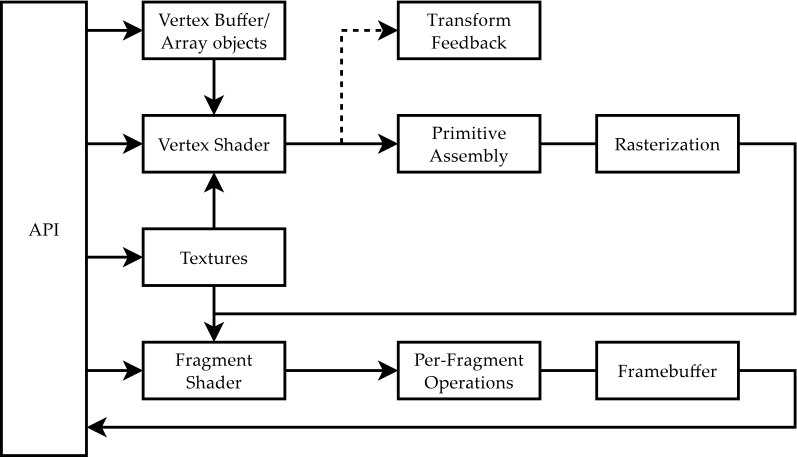
\includegraphics[width=0.8\textwidth]{fig/pipeline}
  \caption{OpenGL~ES pipeline}
  \label{fig:pipeline}
\end{figure}

Both vertices and fragments are automatically shaded in parallel. This
gives rise to a significant performance boost while freeing the
programmer of the burden of coordinating parallel tasks. However,
there are some disadvantages. Shader instances cannot communicate with
each other or reuse previous computations, although some may be cached
behind the scenes. A shader program only specifies a mapping from its
inputs to its outputs; the rest is handled by OpenGL~ES behind the
scenes.

\section{Other frameworks}

OpenGL~ES is not the only API for enabling hardware acceleration. With
the move from serial programming to parallel programming and the
widespread availability of GPU hardware, we have seen the emergence of
several libraries utilizing GPU hardware for general-purpose
programming.

Recall that in OpenGL~ES, each shader runs in isolation and with little
knowledge of how it fits into the larger picture. Furthermore, OpenGL~ES
offers limited support for profiling code. A motivation for using a
general library in place of OpenGL~ES would be to gain more fine-grained
control over parallelized code. Indeed, as we will see in
chapter~\ref{chap:conclusion}, there are some aspects of our
implementation that may benefit from such control.

% The two largest standards are CUDA and OpenCL.

% The following standards are not limited to graphics and provide more
% fine-grained concurrency.

\subsection{CUDA}

% One disadvantage of OpenGL is that there is no parallel linearity.
% Computations cannot be reused across shader invocations.

CUDA (short for Compute Unified Device Architecture) is a parallel
computing API created and backed by Nvidia. It allows both the CPU
(the ``host'') and the GPU (the ``device'') to be programmed in
regular C. Parallel code is written in the form of ``kernels'' that
are spawned on the GPU and may intercommunicate. Furthermore, CUDA
provides fine-grained memory handling: computations may be cached and
reused by other threads. Threads are organized into thread blocks,
which in turn are organized into grids.

% It is Nvidia only.

CUDA is currently officially executable only on CUDA-enabled Nvidia
hardware. It can be run on mobile devices powered by the Tegra chip,
such as the Shield and Google Nexus 9 tablets. While CUDA boasts great
efficiency, this speed is contingent on that the kernel code maxes out
the GPU's resources. This leads to code that is often optimized
towards specific hardware and is not very portable.

CUDA enjoys a huge community, and there are some independent efforts
to make CUDA programming more heterogeneous. A compiler from PGI makes
it possible to use the same CUDA code on x86 processors, Nvidia chips,
or both~\citep{pgi2010:-cuda}. It is also possible to combine CUDA
with OpenGL.

\subsection{OpenCL}

OpenCL is an open and cross-platform standard maintained by the
non-profit Khronos Group. Its parallelization framework is similar to
CUDA's, although the precise terms differ. OpenCL is also more
oriented towards heterogeneous programming, and an OpenCL kernel can
be run on both the CPU and the GPU.

% It is cross-platform, but lower-level than CUDA.

At first glance, as CPUs become more multi-core and ``GPU-like'',
abstracting away their differences behind a common interface seems to
offer an elegant approach to parallel programming. In practice, it is
still necessary to optimize the code for the hardware it is running
on.

% It is somewhat more abstract than CUDA, in that it offers more
% facilities for heterogeneous programming: for instance, OpenCL
% kernels can be run on both the CPU and the GPU.

Thus, with both OpenCL and CUDA, we run into the same paradox: the
development of GPGPU standards was motivated by an aim of uniformity
and portability. However, obtaining good results from parallelized
code is difficult without custom optimization; and optimization makes
the code hardware-specific. In general, it is not possible to create a
low-level API that is cross-platform \emph{and} offers optimal
efficiency at the same time.

Speed-wise, OpenCL is almost on par with CUDA. The hardware support is
broader, and includes mobile devices: OpenCL can be run on a number of
Android phones. The development environment is not as uniform. There
is no single company backing OpenCL, although AMD, ARM and Intel have
declared support for the standard.

% However, this task is quite complex \citep{scarpino12:-opencl}.

As with CUDA, OpenCL can be combined with OpenGL~ES, a task that is
outlined in section~\ref{sec:furtherwork}. However, this is a complex
affair. All in all, little compares to OpenGL~ES in terms of mobile
support and ease of use with regard to graphical problems.

\section{Challenges}
\label{sec:challenges}

In implementing and accelerating barrel undistortion using OpenGL~ES,
we are met with several challenges:
\begin{itemize}
\item To model the distortion in a way that is both efficient and
  produces precise results.
\item To select an implementation strategy that is a good fit for the
  chosen model.
\item To exploit the parallelizable features of the problem to achieve
  good execution speed.
\item To provide high-quality interpolation, adapted to the
  characteristics of the transformation.
\end{itemize}
We will reassess these challenges in chapter~\ref{chap:conclusion}.

\section{Overview}

The structure of the thesis is as follows.
\begin{enumerate}
\item \textbf{Chapter~\ref{chap:introduction}:
    \nameref{chap:introduction}.} This chapter investigates the
  motivation for accelerating image transformation, along with the
  available technologies for doing so.
\item \textbf{Chapter~\ref{chap:trans}: \nameref{chap:trans}.} The
  task of performing fish-eye undistortion is indicative of a larger
  class of problems. In this chapter, we outline a hierarchy of
  transformation problems and investigate their challenges with regard
  to interpolation.
\item \textbf{Chapter~\ref{chap:models}: \nameref{chap:models}.}
  Fish-eye distortion can be modeled in different ways. We compare
  several models and their pros and cons with regard to
  implementation.
\item \textbf{Chapter~\ref{chap:strategies}:
    \nameref{chap:strategies}.} We outline five implementation
  strategies for accelerating fish-eye undistortion. We also describe
  several interpolation methods.
\item \textbf{Chapter~\ref{chap:opengl}: \nameref{chap:opengl}.} The
  aforementioned strategies are implemented with a combination of Qt
  and OpenGL~ES. We describe the class structure and give examples of
  shader code.
\item \textbf{Chapter~\ref{chap:results}: \nameref{chap:results}.} We
  compare the execution times of the implemented strategies. We also
  give visual examples of the interpolation results.
\item \textbf{Chapter~\ref{chap:conclusion}:
    \nameref{chap:conclusion}.} We sum up which strategies give the
  best results. We also highlight some weaknesses and suggest ways to
  improve the efficiency even further.
\end{enumerate}

\section*{Summary}

% OpenGL is the best

Image transformation is a general problem that crops up in different
forms. A particularly well-studied form of the problem is barrel
undistortion, which can be used to correct for the inherent
imprecision of regular lenses or to reverse the ``fish-eye'' effect of
photographs taken with wide-angle lenses. This task raises interesting
challenges with regard to precision, efficiency and quality.

The demand for efficient post-procession of images and video streams
is increasing, as much of that procession takes place on mobile
devices with limited resources. The multi-core imperative has
intensified the need for code that runs fast in parallel.

There are several frameworks for achieving hardware-accelerated
rendering: OpenGL, CUDA and OpenCL. The most widely supported standard
is OpenGL. A recent version, OpenGL~ES, is adapted towards mobile
devices and enjoys widespread support. This is the framework chosen
for our implementation.

\chapter{Image transformation}
\label{chap:trans}

In this chapter we will provide a general discussion of how images can
be transformed. We will first look at how transformations can be
expressed mathematically, and then we will investigate the challenges
with regard to interpolation. In particular, we are interested in the
following issues:
\begin{itemize}
\item How the problem of barrel undistortion fits into the larger
  picture, and to which degree our findings can be generalized to
  other transformations.
\item How the challenges with regard to interpolation depend on the
  complexity of the transformation. Much of the literature discusses
  interpolation techniques in a context of 3D applications. Barrel
  undistortion raises issues that are not addressed in this context.
\item How these transformations can be expressed in OpenGL~ES. The
  shader language and its constructs lends itself well to the class of
  transformations that can be expressed as matrix multiplication, but
  barrel undistortion falls outside this class.
\end{itemize}
We will outline a simple hierarchy of transformations that is roughly
based on the terminology of \citet{wolberg90:-digital-image-warp}.
Then we will discuss various interpolation techniques.

\section{Types of transformation}

\begin{figure}
  \centering
  \subfloat[Scaling]{
    \label{fig:scaling}
    \includegraphics[height=0.1\textwidth]{fig/scaling}
  }
  \qquad\subfloat[Linear transformation]{
    \label{fig:linear}
    \includegraphics[height=0.1\textwidth]{fig/linear}
  }

  \subfloat[Affine transformation]{
    \label{fig:affine}
    \includegraphics[height=0.1\textwidth]{fig/affine}
  }
  \qquad\subfloat[Projective transformation]{
    \label{fig:projective}
    \includegraphics[height=0.1\textwidth]{fig/projective}
  }

  \subfloat[Nonlinear transformation]{
    \label{fig:nonlinear}
    \includegraphics[height=0.1\textwidth]{fig/nonlinear}
  }

  \caption{Transformation types}
  \label{fig:transformations}
\end{figure}

Image transformations can be roughly ordered from simple, linear
transformations to complex, nonlinear transformations
(figure~\ref{fig:transformations}). In the following discussion, we
will consider that each sample in the source image has a coordinate
$[x, y]$, and it is our task to calculate the corresponding position
$[x', y']$ in the transformed image. The problem of blending together
samples in order to produce a smooth output image is postponed to our
treatment of interpolation in section~\ref{sec:interpolation}.

Note that in the following discussion, the transformation takes us
\emph{from} the untransformed coordinates of the source image
\emph{to} the transformed coordinates of the output image. As we will
see later on, it can also be useful to go in the reverse direction.
Many transformations are invertible and can be expressed either way.

\subsection{Scaling}

At the lower end of the spectrum, we have scaling, probably the most
common way of transforming an image. It is very easy to implement and
accelerate, since the neat rows-and-columns shape of the problem lends
itself particularly well to implementation by basic data structures.

Mathematically, scaling can be expressed as multiplying the image
coordinates with a scalar $k$. If the operation is expressed as matrix
multiplication, then the scaling matrix has the form
$[\begin{smallmatrix}
  k & 0\\
  0 & k
\end{smallmatrix}]$, or $k$ times the identity matrix:
\begin{equation}
  \left[\begin{matrix}
      k & 0\\
      0 & k
    \end{matrix}\right]
  \left[\begin{matrix}
      x\\
      y
    \end{matrix}\right]
  =
  \left[\begin{matrix}
      kx\\
      ky
    \end{matrix}\right]
\end{equation}
Of course, scaling is invertible, since scaling by $k$ can be undone
by scaling by $1/k$.

\subsection{Linear transformations}

One step up from scaling, we have linear transformations, such as
rotation, reflection, and shearing. Intuitively, these transformations
can be thought of as ones where parallel lines remain parallel after
transformation.

Mathematically, a transformation $F(\mathbf{x})$ is linear if it preserves the
basic operations of addition and multiplication by a scalar $k$:
\begin{align}
  F(\mathbf{x} + \mathbf{y}) &= F(\mathbf{x}) + F(\mathbf{y})\\
  F(k\mathbf{x}) &= kF(\mathbf{x})
\end{align}
Note that the transformation doesn't shift the coordinate system -- it
maps the zero coordinate onto itself:
\begin{equation}
  \label{eq:zero}
  F(\mathbf{0}) = \mathbf{0}
\end{equation}
Linear transformations can be expressed as multiplication by a
two-by-two matrix $[\begin{smallmatrix}
  m_{11} & m_{12}\\
  m_{21} & m_{22}
\end{smallmatrix}]$.
For all practical purposes, these matrices are invertible, excluding a
few corner cases which are meaningless in the context of image
transformation.

\subsection{Affine transformations}

An affine transformation is a linear transformation followed by
translation, i.e., shifting the coordinate system by offsets $\Delta
x$ and $\Delta y$. Translations cannot be expressed by a two-by-two
matrix, as equation~\eqref{eq:zero} shows. However, if we extend our
two-dimensional coordinates with a ``dummy'' coordinate $z = 1$, we
can express translation as multiplication by a three-by-three matrix:
\begin{equation}
  \left[\begin{matrix}
      1 & 0 & \Delta x\\
      0 & 1 & \Delta y\\
      0 & 0 & 1
    \end{matrix}\right]
  \left[\begin{matrix}
      x\\
      y\\
      1
    \end{matrix}\right]
  = \left[\begin{matrix}
      x + \Delta x\\
      y + \Delta y\\
      1
    \end{matrix}\right]
\end{equation}
An affine transformation can then be expressed as:
\begin{equation}
  \left[\begin{matrix}
      m_{11} & m_{12} & \Delta x\\
      m_{21} & m_{22} & \Delta y\\
      0 & 0 & 1
    \end{matrix}\right]
  \left[\begin{matrix}
      x\\
      y\\
      1
    \end{matrix}\right]
  = \left[\begin{matrix}
      m_{11}x + m_{12}y + \Delta x\\
      m_{21}x + m_{22}y + \Delta y\\
      1
    \end{matrix}\right]
\end{equation}
In actuality, the coordinate $[x, y, z]$ is a \emph{homogeneous}
coordinate. OpenGL~ES provides built-in support for such coordinates,
which extends the scope of transformations that can be expressed as
matrix multiplication.

\subsection{Projective transformations}

If the three-by-three matrix modifies the $z$ coordinate, then the
transformation is projective:
\begin{equation}
  \left[\begin{matrix}
      m_{11} & m_{12} & m_{13}\\
      m_{21} & m_{22} & m_{23}\\
      m_{31} & m_{32} & m_{33}
    \end{matrix}\right]
  \left[\begin{matrix}
      x\\
      y\\
      z
    \end{matrix}\right]
  = \left[\begin{matrix}
      m_{11}x + m_{12}y + m_{13}z\\
      m_{21}x + m_{22}y + m_{23}z\\
      m_{31}x + m_{32}y + m_{33}z
    \end{matrix}\right]
\end{equation}
In this case, the $z$ value contains information. We map from
homogeneous coordinates to image coordinates by dividing by $z$:
\begin{equation}
  \frac{1}{z}
  \left[\begin{matrix}
      x\\
      y\\
      z
    \end{matrix}\right]
  =
  \left[\begin{matrix}
      x/z\\
      y/z\\
      1
    \end{matrix}\right]
\end{equation}
By transforming the input coordinates with this two-step process --
first multiplying with an homogeneous matrix and then mapping back to
two-dimensional coordinates -- we can express more advanced
transformations, for example perspective projection
(figure~\ref{fig:perspective}). Any planar quadrilateral can be
transformed to any other quadrilateral.

\begin{figure}[b]
  \centering
  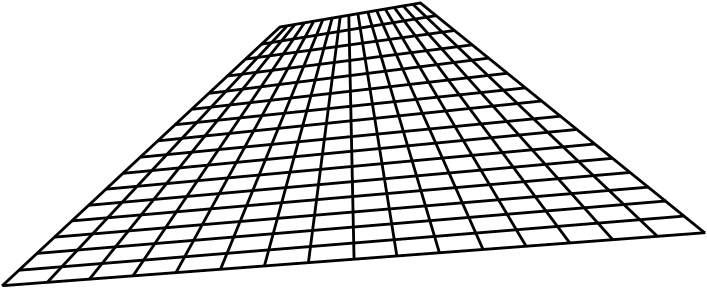
\includegraphics[width=0.5\textwidth]{fig/perspective}
  \caption{Perspective projection}
  \label{fig:perspective}
\end{figure}

In the case of nonplanar quadrilaterals, however, a more general
solution is necessary. The general quadrilateral-to-quadrilateral
problem can be expressed as a bilinear transformation:
\begin{equation}
  \left[\begin{matrix}
      a_3 & a_2 & a_1 & a_0\\
      b_3 & b_2 & b_1 & b_0
    \end{matrix}\right]
  \left[\begin{matrix}
      xy\\
      x\\
      y\\
      1
    \end{matrix}\right]
  =
  \left[\begin{matrix}
      a_3xy + a_2x + a_1y + a_0\\
      b_3xy + b_2x + b_1y + b_0
    \end{matrix}\right]
\end{equation}
For example, a photograph can be transformed from perspective
projection to orthographic projection by mapping a rectangle imaged as
a quadrilateral to a rectangle with the correct aspect
ratio~\citep{zisserman04:-multiple-view}.

% Reference?

% appropriately mapping the outline of a square object in the photograph
% to a flat square on the screen.

% Perspective projection?

Because projective transformations do not distribute samples as
uniformly as simpler transformations do, they tend to present aliasing
issues. A textured surface rendered at an angle as shown in
figure~\ref{fig:perspective}, for example, may introduce artifacts in
the distance. We'll discuss how such effects can be mitigated in our
treatment of interpolation in section~\ref{sec:interpolation}.

\subsection{Nonlinear transformations}
\label{sec:nonlinear}

At an even higher level are the transformations that cannot be
expressed as matrix multiplication at all. We'll refer to this
amorphous class of transformations as ``nonlinear'' transformations.

Barrel distortion, for example, belongs in this class. A coordinate is
skewed depending on its distance from the center. Coordinates near the
margins are moved together, while coordinates near the center are
spread apart. This gives rise to higher frequencies near the margins,
which may produce unwanted aliasing effects.

A nonlinear transformation is not necessarily costly to calculate. If
it is, however, then it might be preferable to compute it in advance
and store it as a table of $[x, y]$-offsets:
\begin{displaymath}
  \left[
    \begin{matrix}
      F(\mathbf{x}_{11}) & F(\mathbf{x}_{12}) & F(\mathbf{x}_{13}) & F(\mathbf{x}_{14}) & \dotsb & F(\mathbf{x}_{1n}) \\
      F(\mathbf{x}_{21}) & F(\mathbf{x}_{22}) & F(\mathbf{x}_{23}) & F(\mathbf{x}_{24}) & \dotsb & F(\mathbf{x}_{2n}) \\
      F(\mathbf{x}_{31}) & F(\mathbf{x}_{32}) & F(\mathbf{x}_{33}) & F(\mathbf{x}_{34}) & \dotsb & F(\mathbf{x}_{3n}) \\
      F(\mathbf{x}_{41}) & F(\mathbf{x}_{42}) & F(\mathbf{x}_{43}) & F(\mathbf{x}_{44}) & \dotsb & F(\mathbf{x}_{4n}) \\
      F(\mathbf{x}_{41}) & F(\mathbf{x}_{42}) & F(\mathbf{x}_{43}) & F(\mathbf{x}_{44}) & \dotsb & F(\mathbf{x}_{4n}) \\
      \vdots             & \vdots             & \vdots             & \vdots             & \ddots & \vdots             \\
      F(\mathbf{x}_{m1}) & F(\mathbf{x}_{m2}) & F(\mathbf{x}_{m3}) & F(\mathbf{x}_{m4}) & \dotsb & F(\mathbf{x}_{mn})
    \end{matrix}
  \right]
\end{displaymath}
Since coordinate transformation is reduced to a single table lookup,
this is very efficient, at least for small tables. For large tables,
cache misses may outweigh the cost of computing the value directly.
Note that if the image resolution is not known beforehand (e.g.,
because of user-adjustable resizing), then this approach requires us
to calculate the table at some sufficiently rich resolution, and then
interpolate between table entries in order to up- or downsample the
table to the given image size. A simple way to achieve this is to
store the table as a texture and let OpenGL~ES interpolate between
texel values.

In general, we are met with two challenges: how to express the
transformation precisely, and how to deal with aliasing effects. Both
are complex problems, and raise a trade-off between quality and
efficiency.

\section{Interpolation}
\label{sec:interpolation}

Thus far, we have only considered how coordinates in the input image
map onto coordinates in the output image. When we work with images, we
encounter the practical problem that continuous coordinates may not
map precisely onto discrete pixels. There may be ``clusters'' and
``gaps'': when enlarging an image, for example, the samples are spread
further apart, leaving empty spaces in between. To produce a smooth
output image, we must perform interpolation.

In the abstract, interpolation can be decomposed into two general
problems: that of reconstructing a discrete image into a continuum,
and that of rasterizing the continuum into a discrete image again.
Transformation is performed in between. Adding an optional filtering
step, the process can be divided into four stages:
\begin{enumerate}
\item \textbf{Reconstruction:} The discrete input $f(x)$ is
  reconstructed into the continuous input $f_c(x)$ with the
  reconstruction filter $r(x)$. This can be expressed as convolution:
  $f_c(x) = f(x) * r(x) = \Sigma_{k} f(x) r(x - k)$. In informal
  terms, the surrounding samples are summed up and weighed according
  to their relative distance to the reconstructed position. A simple
  reconstruction filter may consider only the nearest sample, while a
  more sophisticated filter may compute a weighted average of the
  surrounding area (see section~\ref{sec:filter}).
\item \textbf{Transformation:} The continuous input $f_c(x)$ is
  transformed to $g_c(x)$ according to the transformation function
  $F$. In the case of backward mapping, the transformation is defined
  as an inverse mapping: $g_c(x) = f_c(F^{-1}(x))$. It is also
  possible to perform this step as forward mapping.
\item \textbf{Filtering:} Depending on the transformation, $g_c(x)$
  may contain arbitrarily high frequencies. To prevent aliasing, the
  result may be bandlimited by a filter $h(x)$. Since this step is
  performed in the continuous domain, the convolution is defined as an
  integral: $g_c'(x) = g_x(x) * h(x) = \int g_c(t) h(x -
  t)\,\mathrm{d}t$. In informal terms, high frequencies are smoothed
  out by passing each position through a filter that weighs its
  surroundings.
\item \textbf{Rasterization:} The continuous, transformed, bandlimited
  result $g_c'(x)$ is sampled by $s(x)$, the ``comb function'', to
  produce the discrete output $g(x)$. The ``comb function'' is simply
  defined as $1$ for discrete positions and $0$ otherwise, so that
  sampling can be expressed as multiplication: $g(x) = g_c'(x)s(x)$.
  Note that the output isn't necessarily sampled at the same density
  as that of the input.
\end{enumerate}
In practice, interpolation is usually expressed in more compact terms
(although there are promising efforts to bring a more ``functional''
style into graphics).\footnote{\citet{heard08:-beaut-code} explores
  Haskell's \emph{monad} concept in conjunction with graphics
  processing, giving several examples of how the control flow can be
  abstracted away.} The main point, for our purposes, is that the
transformation is performed either through \emph{forward mapping} or
\emph{backward mapping}. As we will see in chapter~\ref{chap:opengl},
OpenGL~ES lends itself well to both approaches. In the case of a
forward mapping implementation, we go \emph{from} coordinates in the
input image \emph{to} coordinates in the output image
(figure~\ref{fig:forwardmapping}). This is done by constructing a
constructing a grid mesh, transforming it, and then rasterizing the
result. In the case of backward mapping, we go \emph{from} output
coordinates \emph{to} input coordinates
(figure~\ref{fig:backwardmapping}). We therefore make use of the
\emph{inverse} transformation $F^{-1}(\mathbf{x})$, rather than the
original transformation $F(\mathbf{x})$. For example, if the
application is scaling, then instead of scaling coordinates in the
input image by a factor of $k$, we scale coordinates in the output
image by a factor of $1/k$.

\begin{figure}
  \centering
  \subfloat[Forward mapping]{
    \label{fig:forwardmapping}
    \includegraphics[height=0.3\textwidth]{fig/forward}
  }
  \qquad\subfloat[Backward mapping]{
    \label{fig:backwardmapping}
    \includegraphics[height=0.3\textwidth]{fig/backward}
  }

  \caption{Forward mapping and backward mapping}
  \label{fig:forwardandbackwardmapping}
\end{figure}

Which approach is better is a question of context. A complex
transformation may be faster to compute in one direction than the
other. The geometry of the problem may also be exploited to increase
performance. When scaling an image, for example, the interpolation is
usually done in one direction and then in the orthogonal direction
(e.g., first horizontally and then vertically): the first step
produces a set of intermediate values which are blended together in
the second step. But as complex transformations are not geometrically
simple, it is difficult to generalize techniques which depend on the
rows-and-columns shape of the problem. In
section~\ref{sec:adaptiveinterpolation}, we will outline an
interpolation method that is general enough to work well with any
complex transformations, yet flexible enough to be adapted to the
parameters of the transformation.

% Unfortunately, such techniques cannot be generalized to more complex
% transformations.

\subsection{Reconstruction}
\label{sec:filter}

Although interpolation has been expressed as convolution, it is
usually implemented in terms of evaluating the interpolation
polynomial directly at the resampling positions. For example, in the
common case of \emph{bilinear} interpolation, the interpolation is
performed first in one direction, and then again in the orthogonal
direction (thus the interpolation as a whole is actually quadratic,
not linear).

The choice of reconstruction filter has a huge impact on quality and
performance. The simplest filter is the \emph{nearest-neighbor}
filter, which simply copies the value of the nearest sample to the
reconstructed position. This is very efficient (practically a
``no-op''), but tends to yield a blocky and jagged result. In the case
of bilinear interpolation, the \emph{four} ($2 \times 2$) nearest
samples are considered, and a weighted average is computed according
to the proximity to each. Even smoother results can be obtained with
\emph{bicubic} interpolation, although some sharpness of edges gets
lost; this method considers \emph{sixteen} ($4 \times 4$) samples and
is more computationally intensive.\footnote{An even more sophisticated
  choice for resampling is \emph{Lanczos interpolation}, which
  \citet{turkowski90:-graph-gems} considered the ``best compromise in
  terms of reduction of aliasing, sharpness, and minimal ringing''.}
OpenGL~ES contains built-in support for bilinear filtering; other
methods can be implemented as shaders~\citep{bjorke04:-filter}.

% GPU Gems 2

\subsection{Antialiasing}
\label{sec:prefilter}

As we consider more complex transformations, we encounter a new
problem: aliasing. Scaling, linear transformations and affine
transformations are uniform, so that the same quality of interpolation
applies to the whole image. If part of the image is jagged, the whole
image is jagged; if part of the image is smooth, the whole image is
smooth. When we consider projective transformations and beyond, this
no longer holds true. Instead, the ``density'' of the image may vary,
giving rise to high frequencies that, when undersampled, produce
aliasing artifacts.

The ideal way to handle these frequencies would be to sample the image
at a higher resolution. Since this is often prohibitively expensive,
the alternative solution is to get rid of the higher frequencies by
bandlimiting. A crude approach would be to blur the whole image before
transformation. A smarter way is to blur \emph{adaptively}: if we know
where in the image the high frequencies are clustered, we can single
those areas out for adaptive bandlimiting.

In 3D applications, this is often done with a prefiltering technique
known as ``mip-mapping''.\footnote{``Mip'' stands for ``multum in
  parvo'', at Latin phrase meaning ``many things in a small place''.}
The same texture is stored in a range of decreasing resolutions before
use. For example, when a polygon is rendered at an angle,
high-resolution textures may be used for the close parts of the
polygon and low-resolution textures for the distant parts. Anisotropic
filtering builds upon mip-mapping by also downsampling the texture to
nonproportional resolutions.

Prefiltering techniques are optimized for the scenario where the same
image is stored once and rendered many times. When processing a stream
of images on-the-fly, this may not be viable. The following techniques
merge interpolation and antialiasing together in one step.

\subsection{Adaptive interpolation}
\label{sec:adaptiveinterpolation}

One such antialiasing technique is \emph{area sampling}. We may
consider each pixel in the output image to be a square that is mapped
to some shape in the input image, called the ``preimage''. By
computing this area and blending together the samples contained
therein, we obtain a better value for the output. That is, pixels with
a large preimage (and therefore potentially high frequencies) are
sampled at a higher frequency than pixels with a small preimage.

Computing the preimage raises issues on its own, however. As a first
approximation, the coordinates of the four corners of the pixel may be
transformed in reverse to produce the input coordinates of some
approximately quadrilateral shape. For more complex transformations,
the preimage may \emph{not} be quadrilateral at all, and additional
coordinates may be necessary. There is also the recurrent problem that
a ``pixel is \emph{not} a little square'' \citep{smith95:-pixel}. A
pixel is, in fact, a point sample that is rendered in the form of a
little square. This complicates the matter of drawing the line between
samples that are ``inside'' the preimage and samples that are outside
it. In practice, some approximation is necessary.

% Feibush

\begin{figure}
  \centering
  
\includegraphics[width=0.8\textwidth]{fig/supersampling}
  \caption{Supersampling}
  \label{fig:supersampling}
\end{figure}

The technique of \emph{supersampling} sidesteps these geometrical
difficulties (figure~\ref{fig:supersampling}). Instead of dealing
directly with the shape of the preimage, the preimage is merely
``sampled'' a number of times. The value of the output pixel is
computed on the basis of, say, nine ($3 \times 3$) positions that are
overlaid onto the pixel in the form of a uniform grid and then
transformed to input coordinates. These samples are then blended
together.

Supersampling should not be confused with \emph{multisampling}, which
is a built-in anti-aliasing technique provided by OpenGL~ES. If
multisampling is enabled, then each pixel at the edge of a polygon is
sampled multiple times at a slight offset that is smaller than the
pixel size. The samples are averaged together, producing a smoother
edge. However, this does little for the problem of image
transformation, where aliasing artifacts are not confined to polygon
edges. We need to provide a more general method, over whose
implementation we can exert direct control.

% Multisampling, also known as multisample antialiasing (MSAA), is one
% method for achieving full-screen antialiasing (FSAA). With
% multisampling, each pixel at the edge of a polygon is sampled
% multiple times. For each sample-pass, a slight offset is applied to
% all screen coordinates. This offset is smaller than the actual size
% of the pixels. By averaging all these samples, the result is a
% smoother transition of the colors at the edges. Unlike supersampling
% (SSAA) which can result in the same pixel being shaded multiple
% times per pixel, multisampling runs the fragment program just once
% per pixel rasterized. However with MSAA multiple depth/stencil
% comparisons are performed per pixel, one for each of the subsamples,
% which gives you sub-pixel spatial precision on your geometry and
% nice, smoothed edges on your polygons.

As we will see in chapter~\ref{chap:strategies}, supersampling is
simple to implement, but has the cost of increasing the amount of
computations by nine in this case. If the input is a high-resolution
image with lots of detail, then additional samples may be necessary,
making the method increasingly costly. More efficient results can be
obtained by \emph{adaptive supersampling}. We may estimate the size of
the preimage on the basis of a transformed quadrilateral. Large
preimages are supersampled with a higher number of samples, while
small preimages need not be supersampled at all. In this way, adaptive
supersampling improves efficiency.

We can also adapt the way that the samples are blended together, and
thus improve interpolation quality. In the case of barrel
undistortion, we know that the ``sampling density'' depends on the
distance from the center of the image. By building this knowledge into
our interpolation method, we can employ a sharpening filter for
``low-density'' areas and a blurring filter for ``high-density''
areas. Section~\ref{sec:gdbm} describes such a strategy.

\section*{Summary}

Image transformations can be ordered by complexity. Some
transformations can be expressed and implemented as matrix
multiplications, while others require higher-order math. While the
former lends itself well to OpenGL~ES' data structures, the latter may
be costly to compute.

In general, the more complex a transformation is, the harder it is to
interpolate in a way that alleviates aliasing effects. Prefiltering
methods commonly used in 3D applications, where a texture is stored
once and used many times, don't generalize well to the problem of
image transformation. Furthermore, nonlinear transformations may give
rise to uneven aliasing effects. When choosing an interpolation
method, a trade-off between quality and efficiency is raised.

Supersampling is a very adaptable method. The number of samples used
and the way they are blended together can both be adjusted on the
basis of knowledge of the behavior of the transformation.

In the following chapters, we will look at how we can implement
forward mapping and backward mapping in the context of OpenGL~ES, as
well as how we can improve on OpenGL~ES' built-in interpolation with a
supersampling solution. First, however, we will take a closer look at
the problem of modeling barrel distortion.

% To sum up, near-neighbor interpolation considers $1$~pixel, bilinear
% interpolation considers $4$~pixels, and bicubic interpolation
% considers $16$~pixels.

% In the case of \emph{nearest-neighbor interpolation}, the new pixel
% values are computed simply by copying the nearest original pixel.

% \newpage

% The distortion models described in section~\ref{sec:fisheye} are image
% transformations, that is, they are ultimately mappings from one set of
% points to another set of points. For every pixel in the original,
% distorted image, the model gives us the corresponding position of the
% pixel in the new, undistorted image. In general terms, the model is a
% bijective function $f_m\colon \mathbb{R}^2 \to \mathbb{R}^2$ on pixel
% positions:
% \begin{align}
%   \label{eq:function}
%   (x', y') = f_m(x, y),\quad (x, y) = f_m^{-1}(x', y')
% \end{align}
% The consequence of this relocation of pixels may be that some may end
% up closer together, while others end up further apart. To ``fill in''
% the empty spaces in between, we must perform interpolation: that is,
% we must in some way convert our discretized input image into a
% \emph{continuous} range of values, which can then be rasterized (i.e.,
% re-discretized) when producing the output image. Let us consider the
% image itself to be a discrete function $f\colon \mathbb{N}^2 \to
% \mathbb{N}^3$, leaving the details of color representation for
% later.\footnote{See section~\ref{sec:color} for a discussion on color
%   spaces.} We then want to derive a continuous function $g\colon
% \mathbb{R}^2 \to \mathbb{N}^3$:
% \begin{align}
%   \label{eq:image}
%   c_\text{discrete} &= f(x, y),\quad (x, y) \in \mathbb{N}^2\\
%   \label{eq:cont}
%   c_\text{continuous} &= g(x, y),\quad (x, y) \in \mathbb{R}^2
% \end{align}
% There are various ways of deriving $g$ from $f$. Each method of
% interpolation presents a different trade-off between smoothness and
% efficiency. We will first consider these methods in relation to
% scaling an image~\textendash\ where \emph{scaling} is just another
% transformation of the kind described by equation~(\ref{eq:function}).
% Since the pixels retain their relative positions, the new image can
% still be considered in terms of ``rows'' and ``columns'', and this
% geometric fact is easily exploited by efficient scaling
% implementations. However, it no longer holds true when we substitute
% the scaling with a non-uniform transformation, such as a fish-eye
% distortion model. Thus, in the case of scaling or ``resampling'' an
% image, interpolation is usefully seen as a part of the process; but in
% the general case, transforming the image and interpolating it are
% separate steps.

% In the case of \emph{nearest-neighbor interpolation}, the new pixel
% values are computed simply by copying the nearest original pixel. This
% is very efficient (practically a ``no-op''), but tends to yield a
% blocky and jagged result. In the case of \emph{bilinear
%   interpolation}, we consider the \emph{four} ($2 \times 2$) nearest
% source pixels, computing a weighted average according to the proximity
% to each. When resampling an image, the interpolation is usually done
% in one direction and then in the orthogonal direction (e.g., first
% horizontally and then vertically): the first step produces a set of
% intermediate values which are blended together in the second step.
% Smoother results can be obtained with \emph{bicubic interpolation},
% although some sharpness of edges gets lost; this method considers
% \emph{sixteen} ($4 \times 4$) pixels and is more computationally
% intensive.\footnote{An even more sophisticated choice for resampling
%   is \emph{Lanczos interpolation}, which
%   \citet{turkowski90:-graph-gems} considered the ``best compromise in
%   terms of reduction of aliasing, sharpness, and minimal ringing''.}
% To sum up, near-neighbor interpolation considers $1$~pixel, bilinear
% interpolation considers $4$~pixels, and bicubic interpolation
% considers $16$~pixels.

% We now consider interpolation in and of itself. Whether the pixels of
% the source image are transformed in a uniform fashion or not, we can
% still interpolate by picking the closest surrounding pixels to any
% point and blending them together according to the geometric distance
% to each. Such a general interpolation mechanism does not consider the
% image in terms of ``rows'' and ``columns'', but more abstractly as a
% mapping or function from coordinates to color values, like in
% equation~(\ref{eq:image}). The output of the interpolation process is
% a continuous function, like in equation~(\ref{eq:cont}).

% \begin{table}
%   \centering
%   \begin{tabular}{ll}
%     \toprule
%     Discrete image & $f\colon \mathbb{N}^2 \to \mathbb{N}^3$ ($\mathit{DiscImg}$)\\
%     Continuous image & $g\colon \mathbb{R}^2 \to \mathbb{N}^3$ ($\mathit{ContImg}$)\\
%     Interpolation & $f_\mathit{int}\colon \mathit{DiscImg} \to \mathit{ContImg}$\\
%     Transformation & $f_m\colon \mathit{ContImg} \to \mathit{ContImg}$\\
%     Rasterization & $f_\mathit{rast}\colon \mathit{ContImg} \to \mathit{DiscImg}$\\
%     \bottomrule
%   \end{tabular}
%   \caption{The pipeline interface expressed as function types}
%   \label{tab:types}
% \end{table}

% Table~\ref{tab:types} shows how we may regard image transformation and
% interpolation as \emph{higher-order functions}~\textendash\ taking a
% function as input and returning another function as output. Following
% this interpretation, we can outline the pipeline as function
% composition:\footnote{Recall that function composition is read from
%   right to left, so $f_\mathit{rast} \circ f_m \circ f_\mathit{int}$
%   means ``first interpolate, then transform, then rasterize''.}
% \begin{equation}
%   \label{eq:pipeline}
%   f_\mathit{rast} \circ f_m \circ f_\mathit{int}\colon \mathit{DiscImg} \to \mathit{DiscImg}
% \end{equation}
% In a programming language with functional types and lazy evaluation,
% the pipeline could actually be implemented this tersely: data would
% flow from one function to the next according to call-by-need, freeing
% us from the burden of implementing an explicit data
% flow~\citep{heard08:-beaut-code}.\footnote{\citeauthor{heard08:-beaut-code}
%   also gave examples on how the Haskell programming language provides
%   \emph{monads} as a means of abstracting away the control flow, so
%   that one flow can be interchanged for another.} However, in more
% conventional languages with strict semantics \textendash~and when we
% need direct control for efficiency purposes~\textendash\ we must
% handle things ourselves, and equation~(\ref{eq:pipeline}) can only
% serve as a design guideline. To this end, we compare \emph{forward
%   mapping} and \emph{backward mapping}. Other pipeline styles were
% explored by \citet{havard12:-low-sched}.

% In the case of forward mapping, we iterate through the pixels in the
% source image, transform them, and use interpolation to fill in the
% spaces in between. This is easily implemented with OpenGL: for each
% pixel, we create a colored vertex whose position is given by the
% transformation (i.e., $f_m \circ f_\mathit{int}$ is done in one step).
% After tesselation, the fragment shader will simply fill in the areas
% with gradients from one vertex color to another. The result is a
% smooth, interpolated image which can be rasterized at any resolution.

% The reverse approach is backward mapping. In this case, we iterate
% through the pixels of the result image, and then use the
% \emph{inverse} transformation to calculate the corresponding position
% in the source image. This is where the reverse relationships in
% section~\ref{sec:fisheye} come of use. The nearby source pixels are
% interpolated according to their proximity to the calculated position
% (which may not land directly on a source pixel), and this value is
% written to the result image. This is a fairly straightforward way to
% handle interpolation, but an efficient implementation requires a
% distortion model which is fast in inverse.

% There are two main ways to implement an image transformation: forward
% mapping and backward mapping.

% \subsection{Forward mapping}

% In forward mapping, input pixels are mapped to output pixels. For each
% pixel in the input image, one calculates the corresponding position in
% the output image.

% \subsection{Backward mapping}

% In backward mapping, output pixels are mapped in reverse to input
% pixels. For each pixel in the output image, one calculates the
% corresponding original position in the input image.

% \newpage

% \section{Linear transformations}

% Scaling is a linear transformation.

% \subsection{Matrices}

% In OpenGL~ES, linear transformations can be expressed as matrix
% multiplications. In the case of forward mapping, each vertex
% coordinate is multiplied with a transformation matrix. In the case of
% backward mapping, each fragment lookup position is multiplied with a
% reverse transformation matrix.

% \section{Nonlinear transformations}

% Nonlinear transformations cannot be implemented with matrices.

% \subsection{OpenGL~ES mapping}

% OpenGL~ES provides an extensive assortment of mathematical functions
% to implement such transformations.

% \newpage

\chapter{Models of fish-eye distortion}
\label{chap:models}

\begin{figure}[b]
  \centering
  \subfloat[Barrel distortion]{
    \label{fig:barrel}
    \includegraphics[height=0.3\textwidth]{fig/barrel}
  }
  \qquad\subfloat[Pincushion distortion]{
    \label{fig:pincushion}
    \includegraphics[height=0.3\textwidth]{fig/pincushion}
  }

  \caption{Distortion}
  \label{fig:distortion}
\end{figure}

Wide-angle lenses produce a ``fish-eye'' effect, but all lenses
exhibit some degree of barrel distortion. By modeling the distortion
precisely, it is possible to undistort the image, producing a
``pincushion'' effect instead. In this way, we can correct for the
inherent imprecision of regular lenses, as well as for the
``fish-eye'' effect of wide-angle images.

Barrel distortion and pincushion are illustrated in
figure~\ref{fig:distortion}. Observe that in the case of barrel
distortion, the ``density'' of the lines increases towards the edges.
In the case of pincushion distortion, on the other hand, the reverse
is true: the center of the image has the highest ``density''. It is
this area that is prone to aliasing effects when undistorting a
high-frequency image.

The main challenge is to model the distortion precisely. Mitigating
the ``fish-eye'' effect of a wide-angle lens can be done on the basis
of known lens parameters. Correcting for the inherent imprecision of a
normal lens, on the other hand, requires more fine-grained parameters
measured by a calibration routine. These parameters must then be fed
into an equation that is precise enough to undo the distortion,
without introducing additional distortion of its own.

When we compare models, we encounter a trade-off between precision and
efficiency. If only approximate results are needed, then undistorting
an image requires little computing power, and can be modeled in many
ways. \emph{Precisely} modeling the distortion is another matter. Not
only are the precise models more costly; unfortunately, they are also
less mathematically tractable than the simpler models.

\section{Polar coordinates}

Barrel distortion is most easily expressed in polar coordinates, with
the center of the lens at the center of the coordinate system.
OpenGL~ES, however, uses Cartesian coordinates. Luckily, it is not
necessary to perform coordinate conversion to and from polar
coordinates in order to calculate the distortion. In this section, we
will derive a \emph{displacement factor} that lets us compute the
distortion in Cartesian space (figure~\ref{fig:displacement}).

\begin{figure}[b]
  \centering
  \subfloat[Cartesian coordinates]{
    \label{fig:cartesian}
    \includegraphics[width=0.3\textwidth]{fig/cartesian}
  }
  \quad\subfloat[Polar coordinates]{
    \label{fig:polar}
    \includegraphics[width=0.3\textwidth]{fig/polar}
  }

  \caption{Displacement}
  \label{fig:displacement}
\end{figure}

If $[x, y]$ are the Cartesian coordinates of a point, then the polar
coordinates $[r, \theta]$ represent the radius $r$ and the angle
$\theta$ with the positive $x$ axis. The relationship between
Cartesian coordinates and polar coordinates is:
\begin{equation}
  \label{eq:cartesiantopolar}
  % \! typographical correction
  [r, \theta] = \left[\!\sqrt{x^2 + y^2}, \atantwo(y, x)\right]
\end{equation}
where $\atantwo$ is the arcus tangent function of \emph{two} arguments
$y$ and $x$, which expresses the quadrant of the angle
accurately.\footnote{This is provided as the \lstinline|atan()|
  function in OpenGL~ES.} The inverse relationship is given by:
\begin{equation}
  \label{eq:polartocartesian}
  [x, y] = [r\cos{\theta}, r\sin{\theta}]
\end{equation}
A model is a mapping from an untransformed coordinate $[r, \theta]$ to
a transformed coordinate $[r', \theta']$. (It may map undistorted
coordinates to distorted coordinates or vice versa; for the time
being, we ignore the direction of the model and only concern ourselves
with the mapping itself.) Since the angle doesn't change (i.e.,
$\theta' = \theta$), the model can be expressed more compactly as the
relationship between the undistorted radius $r$ and the distorted
radius $r'$:
\begin{equation}
  \label{eq:model}
  r' = F(r)
\end{equation}
We can avoid incurring the cost of the trigonometric functions in
equations~(\ref{eq:cartesiantopolar}--\ref{eq:polartocartesian}). Let
$d$ be the displacement factor, expressed as the ratio of the
distorted radius to the undistorted radius:
\begin{equation}
  \label{eq:displacement}
  d = \frac{r'}{r} = \frac{F(r)}{r}
\end{equation}
Then the relationship between undistorted polar coordinates and
distorted polar coordinates can be expressed in terms of this factor:
\begin{equation}
  \label{eq:polardisplacement}
  [r', \theta'] = [F(r), \theta] = \left[\frac{F(r)}{r}r, \theta\right] = [dr, \theta]
\end{equation}
Likewise, the relationship between undistorted Cartesian coordinates and
distorted Cartesian coordinates is given by:
\begin{equation}
  \label{eq:cartesiandisplacement}
  [x', y'] = d[x, d] = [dx, dy]
\end{equation}
This is easily verified by substituting
equation~(\ref{eq:polardisplacement}) into
equation~(\ref{eq:polartocartesian}). In the rest of the chapter, we
will consider distortion to be a function of the radius.

% In the rest of the chapter, we will work with polar coordinates.

\section{Polynomial models}

The classical distortion model is Brown's model. In addition to radial
distortion, it also models tangential distortion, which occurs when
the lens is not aligned with the sensor. The model is commonly
approximated as a Taylor series:
\begin{equation}
  \label{eq:brown}
  \begin{split}
    x_u &= x_d + (x_d - x_c)(\kappa_1r^2 + \kappa_2r^4 + \kappa_3r^6 + \dotsb) + {} \\
    &\phantom{{}={}} [(\rho_1(r^2 + 2(x_d - x_c)^2) + 2\rho_2(x_d - x_c)(y_d - y_c))(1 + \rho_3r^2 + \dotsb)]\\
    y_u &= y_d + (y_d - y_c)(\kappa_1r^2 + \kappa_2r^4 + \kappa_3r^6 + \dotsb) + {} \\
    &\phantom{{}={}} [(\rho_1(r^2 + 2(y_d - y_c)^2) + 2\rho_2(y_d - y_c)(y_d - y_c))(1 + \rho_3r^2 + \dotsb)]
  \end{split}
\end{equation}
where $[x_u, y_u]$ is the undistorted image point, $[x_d, y_d]$ is the
distorted image point, $[x_c, y_c]$ is the center of distortion (i.e.,
$[0, 0]$ under our assumptions), $\kappa_n$ is the $n$th radial distortion
coefficient and $r$ is the radius as defined in
equation~(\ref{eq:cartesiantopolar}). The part in brackets expresses
tangential distortion, where $\rho_n$ is the $n$th tangential distortion
coefficient.

If we substitute $[x_c, x_c] = [0, 0]$ and remove the tangential part,
the model simplifies to:
\begin{equation}
  \label{eq:brownradial}
  \begin{split}
    x_u &= x_d(1 + \kappa_1r^2 + \kappa_2r^4 + \kappa_3r^6 + \dotsb)\\
    y_u &= y_d(\underbrace{1 + \kappa_1r^2 + \kappa_2r^4 + \kappa_3r^6 + \dotsb}_d)
  \end{split}
\end{equation}
where $d$ is the displacement factor we defined in
equation~(\ref{eq:displacement}). Since the polynomial $d = f(r)$ must
be symmetric in $r$, only the coefficients of even powers of $r$ will
be nonzero. Higher-order terms contribute very little, so
equation~(\ref{eq:brownradial}) can be approximated by a finite
expression where the coefficient $\kappa_1$ controls the general
behavior of the distortion:
\begin{equation}
  \label{eq:taylorone}
  d = f(r) = 1 + \kappa_1r^2
\end{equation}
The coefficient $\kappa_2$ needs only be added if a first-order
approximation is insufficient:
\begin{equation}
  \label{eq:taylortwo}
  d = f(r) = 1 + \kappa_1r^2 + \kappa_2r^4)
\end{equation}
However, for larger distortions (i.e., wide-angle lenses), at least
three terms are needed:
\begin{equation}
  \label{eq:taylorthree}
  d = f(r) = 1 + \kappa_1r^2 + \kappa_2r^4 + \kappa_3r^6
\end{equation}
Brown's model is a mapping from distorted positions to undistorted
positions, i.e., a relationship of the form $[x_u, y_u] = F(x_d,
y_d)$. This allows us to determine where any point in the distorted
image would appear if there was \emph{no} lens distortion. Applied as
a forward mapping image transformation, it produces a ``pincushion''
effect (the opposite of barrel distortion). However, lens undistortion
can also be implemented in terms of the reverse relationship, $[x_d,
y_d] = F^{-1}(x_u, y_u)$, provided we substitute backward mapping for
forward mapping. Table~\ref{tab:mappings} shows the relationships
between interpolation method, model direction, and the produced
effect.

\begin{table}
  \centering
  \begin{tabular}{@{}lll@{}}
    \toprule
    Interpolation & Model & Effect \\
    \midrule
    Forward mapping & $[x_u, y_u] = F(x_d, y_d)$ & Pincushion \\
    Backward mapping & $[x_u, y_u] = F(x_d, y_d)$ & Barrel \\
    Forward mapping & $[x_d, y_d] = F^{-1}(x_u, y_u)$ & Barrel \\
    Backward mapping & $[x_d, y_d] = F^{-1}(x_u, y_u)$ & Pincushion \\
    \bottomrule
  \end{tabular}

  \caption{Forward mapping and backward mapping}
  \label{tab:mappings}
\end{table}

If we want to implement a backward mapping image transformation in
terms of the inverse relationship, we encounter the problem that
equation~(\ref{eq:taylorthree}) has no closed-form solution. If
precision is less of a concern, we can precompute the mapping and
store the values in a table, as outlined in
section~\ref{sec:nonlinear}. However, methods like supersampling are
likely to request a position that is not stored in the table,
requiring us to interpolate between table entries.

Another approach is to compute the inverse by an iterative method such
as Newton--Raphson approximation:
\begin{equation}
  \label{eq:newton}
  x_{n+1} = x_n - \frac{f(x_n)}{f'(x_n)}
\end{equation}
To approximate a value for $r$ corresponding to a displacement $d$, we
rewrite equation~(\ref{eq:taylorthree}) on the form $f(r) = 0$:
\begin{equation}
  \label{eq:rewrite}
  f(r) = 0 = 1 + \kappa_1r^2 + \kappa_2r^4 + \kappa_3r^6 - d
\end{equation}
The derivative of this polynomial is:
\begin{equation}
  \label{eq:derivative}
  f'(r) = 2\kappa_1r + 4\kappa_2r^3 + 6\kappa_3r^5
\end{equation}
Substituting equations~(\ref{eq:rewrite}--\ref{eq:derivative}) into
equation~(\ref{eq:newton}) gives us:
\begin{equation}
  \label{eq:approximation}
  r_{n+1} = r_n - \frac{1 + \kappa_1r^2 + \kappa_2r^4 + \kappa_3r^6 - d}{2\kappa_1r + 4\kappa_2r^3 + 6\kappa_3r^5}
\end{equation}
This is an iterative equation for finding better and better estimates
of $r$ such that $f(r) = d$. Since the equation is considerably more
complicated than the forward relationship, we would like to reduce the
number of iterations to a minimum. Note that the approximation
converges towards better estimates depending on how good the previous
estimate was. Thus, by combining Newton--Raphson approximation with
precomputed values in a table, the number of iterations can be
reduced. The initial estimate is picked from a precomputed table $T$,
and subsequent iterations refine it. Algorithm~\ref{alg:newton}
illustrates this approach.

\begin{algorithm}[h]
  \caption{Newton--Raphson approximation}
  \label{alg:newton}
  \begin{algorithmic}
    \STATE $r \leftarrow T(d)$ \COMMENT{initial estimate from table}
    \FOR{$n = 0$ \TO $N$}
    \STATE $r \leftarrow r - \tfrac{1 + \kappa_1r^2 + \kappa_2r^4 +
      \kappa_3r^6 - d}{2\kappa_1r + 4\kappa_2r^3 + 6\kappa_3r^5}$
    \COMMENT{refine estimate}
    \ENDFOR
    \RETURN $r$ \COMMENT{final estimate}
  \end{algorithmic}
\end{algorithm}

In general, Brown's model is cheap in one direction, but costly in the
other direction. That makes it a less than optimal choice for backward
mapping implementations with advanced interpolation methods, since in
addition to the cost of interpolation, we also get the cost of
approximating the model's inverse. If precision is less of a concern,
then an alternative is to use a less precise model which is easier to
invert. There are several such models to choose from.

% Note that while equation~(\ref{eq:taylorthree}) expresses the displacement
% from distorted to undistorted positions

% This is a \emph{radial} form of distortion, being zero at the center
% of the lens and varying as one moves outward.

% A wide-angle lens produces a ``fish-eye'' effect commonly known as
% \emph{barrel distortion}. This is a \emph{radial} form of
% distortion, being zero at the center of the lens and increasing as
% one moves outward. Even regular lenses tend to exhibit a small
% degree of barrel distortion near the edges.

\section{Non-polynomial models}

\subsection{Exponential model}
\label{sec:exponential}

% We then want to define a mapping from a distorted coordinate $(r,
% \theta)$ to an undistorted coordinate $(r', \theta')$, where $\theta'
% = \theta$ assuming the distortion is symmetrical. (In some cameras,
% pixels are rectangular, but we will overlook this complication here.)

\citet{schwarz80:-comput} showed that the relationship between the
distorted radius $r_d$ and the undistorted radius $r_u$ can be
approximated by the following exponential equation:
\begin{equation}
  \label{eq:exp}
  r_u = (\mathrm{e}^{r_d/s} - 1) / \lambda
\end{equation}
where $s$ is a scaling factor and $\lambda$ is the amount of
distortion. The \emph{inverse} relationship is given by a logarithmic
equation:
\begin{equation}
  \label{eq:logarithm}
  r_d = s\ln(1 + \lambda r_u)
\end{equation}
\citet{basu95:-alter} compared this model with a polynomial model, and
found it to produce good results.

% More models were explored by \citet{basu95:-alter}.

% As we shall see in section~\ref{sec:interpolation}, \emph{both}
% relationships will come in handy in the context of interpolation.

\subsection{Trigonometric model}

% However, \citet{shah96:-intrin} showed that this may not be
% sufficient; in extreme cases, distortion still remains even with a
% third-order distortion model.

\citet{devernay01:-straig-lines} proposed an alternate approximation:
\begin{align}
  \label{eq:devernay}
  r_u &= \tfrac{1}{\omega} \atan(2r_d\tan{\tfrac{\omega}{2}})\\
  r_d &= \frac{\tan(r_u\omega)}{2\tan{\tfrac{\omega}{2}}}
\end{align}
where $\omega$ is the field-of-view of the corresponding ideal
wide-angle lens.

% More models were explored by \citet{basu95:-alter}.

\subsection{Division model}

\citet{fitzgibbon01:-simul} described a fast inverse model called the
``division model'':
\begin{equation}
  \label{eq:division}
  r_d = \frac{1}{1 + \kappa r^2}r_u
\end{equation}
This model is about as good an approximation as the first-order Taylor
expansion in equation~{\ref{eq:taylorone}}, but in the opposite
direction.

\section{Parameter estimation}

The coefficients of the models can be fitted to a curve using the
least squares method. In the case of polynomial models,
\citet{basu95:-alter} showed that the resulting set of linear
equations can be solved by an analytical method such as Gauss--Jordan
elimination.

In the case of non-polynomial models, there is no simple relationship
between the parameters of one model and the parameters of another.
Therefore, analytical methods are not applicable. Instead, the
parameters can be estimated with successive evaluation techniques such
as Newton--Raphson approximation.

Using Matlab's \lstinline|fitnlm()| function, we obtained the
following coefficients for Brown's model:\footnote{The complete Matlab
  code is given in Appendix~\ref{chap:matlab}.}
\begin{equation}
  \label{eq:taylorparam}
  d = f(r) = 1 - 3.5778r^2 + 7.1946r^4 + -3.9842r^6
\end{equation}
For the exponential model:
\begin{align}
  \label{eq:expparam}
  r_u &= (\mathrm{e}^{r_d/0.76} - 1) / 3.8342\\
  \label{eq:logparam}
  r_d &= 0.76\ln(1 + 3.8342r_u)
\end{align}
For the trigonometric model:
\begin{align}
  \label{eq:devernayparam}
  r_u &= \tfrac{1}{0.95617} \atan(2r_d\tan{\tfrac{0.95617}{2}})\\
  r_d &= \frac{\tan(0.95617r_u)}{2\tan{\tfrac{0.95617}{2}}}
\end{align}
For the division model:
\begin{equation}
  \label{eq:divisionparam}
  r_d = \frac{1}{1 - 0.29948r^2}r_u
\end{equation}

\section*{Summary}

Fish-eye distortion can be modeled in various ways. Polynomial models
offer high precision, and are a good choice for forward mapping
implementations. In the case of backward mapping implementations,
however, polynomial models are expensive to invert, requiring
precomputed tables in combination with interpolation methods or
iterative approximation. If loss of precision is acceptable, then
non-polynomial models are a better fit for backward mapping
implementations.

While there are no straightforward relationships between the
parameters of one model and another, the coefficients can be estimated
with nonlinear regression.

% \citet{vamsidhar14:-inter-zoom} implemented controls for interactive
% zooming and panning of wide-angle images.

% \chapter{Implementations of mathematical functions}

% \section{C functions}

% \section{Mantissa and exponent}

% \section{Comparing mathematical models}

% \part{The project}

\chapter{Implementation strategies}
\label{chap:strategies}

So far, we have considered how image transformation can be expressed
mathematically, the challenges it raises with regard to interpolation,
and what models we may use to express fish-eye distortion. In this
chapter, we will consider various strategies for implementing such
distortion using OpenGL~ES.

\section{Implementation considerations}

There are several factors to consider:
\begin{enumerate}
\item \textbf{CPU or GPU:} Whether we want to calculate the
  distortion on the CPU, or accelerate it with the GPU.
\item \textbf{Precomputed or dynamic:} Whether we want to store the
  transformation in a lookup table, or compute it mathematically.
\item \textbf{Forward mapping or backward mapping:} Whether we compute
  output coordinates in terms of input coordinates (forward mapping),
  or input coordinates in terms of output coordinates (backward
  mapping).
\item \textbf{Built-in or manual interpolation:} Whether we rely on
  OpenGL~ES' built-in interpolation methods, or implement our own.
\end{enumerate}
Let us discuss each of these items in detail.

\subsection{CPU or GPU}

An OpenGL~ES pipeline uses both the CPU and the GPU to some extent
(figure~\ref{fig:flow}). However, the brunt of the workload can be
computed by the CPU, or it can be accelerated by the GPU.

\begin{figure}
  \centering
  \includegraphics[width=0.9\textwidth]{fig/cpuandgpu}
  \caption{Data flow}
  \label{fig:flow}
\end{figure}

The transformation may be programmed in C (or in our case, in C++) and
computed entirely by the CPU. If a vertex mesh is used to transform
the image, this mesh needs only be computed once, and can be reused
many times. The task of OpenGL~ES is then to apply a texture to this
mesh and interpolate the result.

Alternatively, the transformation may be programmed in shader code and
computed by the GPU. Since each coordinate can be transformed without
relation to the others, the whole task is ``embarrassingly parallel'',
and easy to code in terms of shaders. Furthermore, this approach is
more flexible in that it can be combined with a custom interpolation
technique.

\subsection{Precomputed or dynamic}

There are several ways of caching the computations for later use.
Transforming a vertex mesh entirely on the CPU is one strategy. Hybrid
approaches are also possible: the CPU may compute a lookup table which
is used by the shader. To obtain continuous values, the shader may
interpolate between table entries, or use the closest table entry to
seed an estimation method such as Newton--Raphson approximation.

\subsection{Forward mapping or backward mapping}

If the image is transformed by applying a texture to a grid mesh,
there is a mapping between vertex positions and texture coordinates. A
forward mapping implementation transforms the vertex positions; a
backward mapping implementation transforms the texture coordinates.
This transformation can be computed by the CPU or in the vertex
shader.

Alternatively, a backward mapping implementation may be implemented in
the fragment shader. In such an implementation, each pixel in the
output image is computed by determining the corresponding position in
the input image and sampling it.

\subsection{Built-in or manual interpolation}

% Our case study will be an implementation of fish-eye transformation
% using a combination of Qt C++ and OpenGL~ES. The code for the
% implementation is available from a Git repository (see
% Appendix~\ref{chap:code}).

% In this chapter, we compare various implementations of image
% transformation using a combination of Qt C++ and OpenGL~ES. The code
% for the implementation is available from a Git repository (see
% Appendix~\ref{chap:code}).

% Implementing image transformation can be done in several ways.

OpenGL~ES provides built-in bilinear interpolation. This option is very
fast and yields reasonable results. It also simplifies the
implementation; all that needs to be coded is the mathematical
relationship of the image transformation.

Alternatively, more sophisticated means of interpolation can be
implemented manually, at the cost of more code and more computations.
We will explore how interpolation can be performed in the fragment
shader.

% ref

\section{Implementation strategies}

As we can see, we have several options when implementing image
transformation. Table~\ref{tab:strategies} lists some possible
\emph{interpolation strategies} -- that is, ways of combining these
options. Some options tend to go together with other options, but the
table is not exhaustive; many other combinations are possible. In this
section, we will focus on a selection of implementation strategies to
illustrate the possibilities.

\begin{table}
  \centering
  \footnotesize
  \begin{tabular}{@{}lllll@{}}
    \toprule
    & Acceleration: & Computation: & Mapping: & Interpolation: \\
    & \underline{C}PU/\underline{G}PU &
    \underline{P}recomputed/\underline{D}ynamic &
    \underline{F}orward/\underline{B}ackward &
    \underline{B}uilt-in/\underline{M}anual \\
    \midrule
    1 & C & P & F & B \\
    2 & C & P & B & B \\
    3 & G & D & F & B \\
    4 & G & D & B & B \\
    5 & G & D & B & M \\
    \bottomrule
  \end{tabular}

  \caption{Implementation strategies}
  \label{tab:strategies}
\end{table}

\subsection{Strategy 1: CPFB}

\begin{figure}[b]
  \centering
  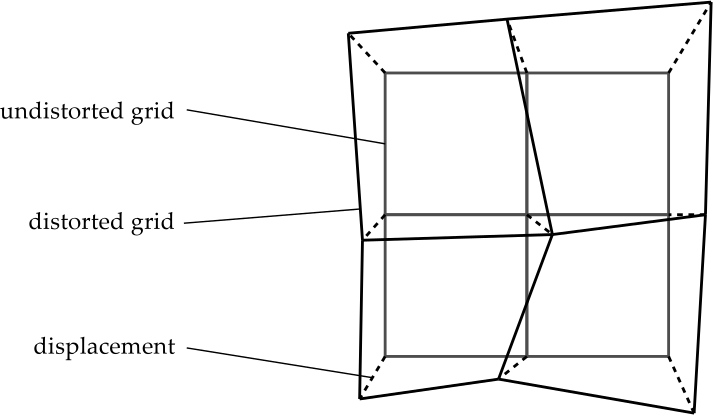
\includegraphics[width=0.6\textwidth]{fig/gridmapping}
  \caption{Transformation grid}
  \label{fig:gridmapping}
\end{figure}

The first strategy computes the transformation on the CPU (C),
precomputes the transformation before use (P), employs forward mapping
(F), and uses OpenGL~ES' built-in interpolation (B). This is done by
loading the image as a texture which is projected onto a transformed
grid mesh. The crucial insight is that the mesh needs only be
transformed once, and can be reused many times (e.g., when
transforming a video sequence). If the image size is known in advance,
the mesh need not even be computed when running the program; it can be
stored as precomputed data.

% \section{Overview}

% When we perform image transformation in OpenGL~ES, we will load the
% image as a texture which is then projected onto a grid mesh. The
% transformation can be performed in a number of ways. For example,
% \citet{mcreynolds05:-advanced} suggests to transform the mapping from
% vertex space to texture space in reverse. There are many possible
% approaches: we can perform forward mapping or backward mapping; the
% transformation may occur in C++ or in shader code; it may be
% calculated on-the-fly or be cached in advance.

The strategy uses forward mapping, since the shape of the mesh is
transformed directly. We can think of it like this: we create a grid
mesh of, say, $10 \times 10$ vertices. Each vertex is mapped to a
corresponding coordinate in texture space: the bottom-left vertex is
mapped to the bottom-left corner of the texture, the upper-right
vertex is mapped to the upper-right corner, and so on. Then the
positions of the vertices are transformed by means of the chosen
model. In consequence, the texture is warped.

As illustrated in figure~\ref{fig:gridmapping}, the transformation is
a mapping from regular rectangles (the undistorted grid) to
quadrilaterals (the distorted grid). Although the vertex positions
have changed, the texture coordinates still map to the undistorted
grid.

The strategy leaves interpolation to OpenGL~ES. The smoothest results
are achieved by OpenGL~ES' \lstinline|GL_LINEAR| option. Some versions
also supports multisampled anti-aliasing, although this is
considerably more expensive. However, since the strategy is very
efficient in the first place, the impact may be negligible.

\subsection{Strategy 2: CPBB}

The second strategy is like the first, but employs backward mapping
instead (B). This is done by transforming the other end of the mapping
between vertex positions and texture coordinates. That is, while the
forward mapping strategy transformed the vertex positions and held the
texture coordinates constant, the backward mapping strategy transforms
the texture coordinates and holds the vertex positions constant
\citep{mcreynolds05:-advanced}.

To explain this transformation in detail, we need to give an overview
of OpenGL~ES' coordinate spaces. By itself, OpenGL~ES contains a
mapping between \emph{two} coordinate spaces: vertex positions $[x,
y]$ in the range $[-1, 1]$ and texture coordinates $[s, t]$ in the
range $[0, 1]$. The default mapping is given by the equation:
\begin{equation}
  \label{eq:mapping}
  \left[\begin{matrix}
      s\\
      t
    \end{matrix}\right]
  =
  \left[\begin{matrix}
      x/2 + 1/2\\
      y/2 + 1/2
    \end{matrix}\right]
\end{equation}
This is an affine transformation, where vertex space is centered
around $[0, 0]$. It is translated and scaled to texture space, which
is centered around $[1/2, 1/2]$. Using the conventions established in
chapter~\ref{chap:trans}, we can express the translation in matrix
form:
\begin{equation}
  \label{eq:affinemapping}
  \left[\begin{matrix}
      s\\
      t\\
      1
    \end{matrix}\right]
  =
  \left[\begin{matrix}
      x\\
      y\\
      1
    \end{matrix}\right]
  \left[\begin{matrix}
      1/2 & 0 & 1/2\\
      0 & 1/2 & 1/2\\
      0 & 0 & 1
    \end{matrix}\right]
\end{equation}
Or in tableaux form:
\begin{equation}
  \label{eq:table}
  \left[\begin{matrix}
      s\\
      t
    \end{matrix}\right]
  =
  \begin{cases}
    [0, 0] & \text{if $[x, y] = [-1, -1]$}\\
    [0, 1] & \text{if $[x, y] = [-1, 1]$}\\
    [1, 0] & \text{if $[x, y] = [1, -1]$}\\
    [1, 1] & \text{if $[x, y] = [1, 1]$}\\
    [1/2, 1/2] & \text{if $[x, y] = [0, 0]$}\\
    \dots & \\
    [x/2 + 1/2, y/2 + 1/2] &
  \end{cases}
\end{equation}
The inverse relationship is of course given by:
\begin{equation}
  \label{eq:inversemapping}
  \left[\begin{matrix}
      x\\
      y
    \end{matrix}\right]
  =
  \left[\begin{matrix}
      2(s - 1/2)\\
      2(t - 1/2)
    \end{matrix}\right]
\end{equation}
The utility of equations~\ref{eq:mapping}--\ref{eq:inversemapping} is
evident when we want to transform texture space. The transformation
equations assume that the coordinate space is centered around $[0,
0]$, \emph{not} $[1/2, 1/2]$. Therefore we must translate the
coordinates before and after conversion, as shown in
algorithm~\ref{alg:coord}.

\begin{algorithm}[h]
  \caption{Coordinate conversion}
  \label{alg:coord}
  \begin{algorithmic}
    \STATE $[x, y] \leftarrow [2(s - 1/2), 2(t - 1/2)]$ \COMMENT{convert to vertex space}
    \STATE $[x', y'] \leftarrow F([x, y])$ \COMMENT{transform coordinates}
    \STATE $[s', t'] \leftarrow [x'/2 + 1/2, y'/2 + 1/2]$ \COMMENT{convert to texture space}
  \end{algorithmic}
\end{algorithm}

Aside from these caveats, the implementation is straightforward and
yields comparable results to the first strategy. The additional
computations introduced by the coordinate conversion in
algorithm~\ref{alg:coord} are negligible and do not contribute much to
the overall cost. Which is the better choice? It depends. If all
necessary parameters are known beforehand so that the whole mesh can
be stored as precomputed data, it doesn't really matter whether we
choose one or the other. However, if the image size is not known and
the mesh needs to be computed as least once when the program is
initialized, then backward mapping may be preferable over forward
mapping \emph{if the chosen model is faster in that direction}. As we
saw in chapter~\ref{chap:models}, models differ in this regard: a
model well-suited for a forward mapping strategy may be a poor choice
for a backward mapping strategy, or vice versa. If there is an
``impedance mismatch'' between model and strategy, we should change
one or the other.

% As we will see, the image transformation can be \emph{grafted} onto
% the vertex--texture mapping in several ways. If we hold the texture
% coordinates constant, but transform the vertex positions they map
% onto, we perform forward mapping. If we hold the vertex positions
% constant and transform the texture coordinates, we perform backward
% mapping.

% This would be an instance of forward mapping: the vertices of the
% grid are changed to their transformed counterparts.

% An example of backward mapping would be to keep the grid mesh
% unchanged, but transform the vertex coordinates the grid maps onto.
% This approach would make use of the inverse transformation.

\subsection{Strategy 3: GDFB}

The previous strategies have left little work to be performed by the
GPU. For anything to be rendered, OpenGL~ES requires us to at least
write a simple vertex shader that passes the vertex data through
unchanged (assuming that the input coordinates matches the screen
coordinates), and a fragment shader that samples the color of the
texture at the given coordinate.

We can move the transformation into these very shaders. As before, we
first create a regular grid mesh of, say, $10 \times 10$ vertices.
Then we pass each vertex to the vertex shader, letting the vertex
shader compute the transformed position. The end result is the same as
when performing forward mapping on the CPU, but the transformation is
expressed in shader code instead.

If this approach is applied to a video sequence, the consequence is
that the transformation is re-computed for each frame. To avoid this,
the grid may be transformed by a separate vertex shader that is run
only once and whose results are saved for later use. OpenGL~ES 3.0
allows the output of a shader to be captured in a buffer object. The
rendering itself is performed by a simple pass-through shader, as in
the CPU case.

\subsection{Strategy 4: GDBB}
\label{sec:implementationgdbb}

Backward mapping can also be done on the GPU. Whereas forward mapping
was performed by the vertex shader, backward mapping is more
appropriately performed by the fragment shader. The reason is that in
this case, we don't need a $10 \times 10$ grid mesh -- a simple
quadrilateral of four vertices will suffice. The task of the fragment
shader, which is run once per output pixel in this case, is to
transform the corresponding texture coordinate before sampling the
texture at that coordinate.

As in the CPU case, we must perform coordinate conversion before and
after the transformation. We must also check if the transformation
returns a position that is out of range: if so, we return a blank
color (e.g., white). Section~\ref{sec:implementationgdbb} describes
the implementation of such a coordinate check.

\subsection{Strategy 5: GDBM}
\label{sec:gdbm}

All the previous strategies have relied on built-in interpolation.
However, the last strategy, which performs backward mapping on the
GPU, can be combined with supersampling as a custom interpolation
step. Instead of sampling a \emph{single} color value, which will have
been interpolated for us by OpenGL~ES' \lstinline|GL_LINEAR| option,
we can sample multiple values and blend them together ourselves. If we
know that the length and height of an output pixel is $l$, then the
positions of the corners are given as follows:
\begin{align}
  \label{eq:ul}
  [x, y]_{ul} &= [x - \tfrac{1}{2}l, y + \tfrac{1}{2}l] \\
  [x, y]_{ur} &= [x + \tfrac{1}{2}l, y + \tfrac{1}{2}l] \\
  [x, y]_{ll} &= [x - \tfrac{1}{2}l, y - \tfrac{1}{2}l] \\
  [x, y]_{lr} &= [x + \tfrac{1}{2}l, y - \tfrac{1}{2}l]
\end{align}
These four coordinates plus the original coordinate can then be
transformed to input coordinates that are sampled to compute an
average of five values. Alternatively, we can overlay a grid of $3
\times 3$ positions over the pixel and sample the input at nine
different positions. This gives us four more positions to compute:
\begin{align}
  [x, y]_{um} &= [x, y + \tfrac{1}{2}l] \\
  [x, y]_{ml} &= [x - \tfrac{1}{2}l, y] \\
  [x, y]_{mr} &= [x + \tfrac{1}{2}l, y] \\
  \label{eq:lm}
  [x, y]_{lm} &= [x, y - \tfrac{1}{2}l]
\end{align}
An unweighed average produces a smooth, if somewhat fuzzy result. We
can achieve a different filtering effect by adjusting the
coefficients~-- that is, by computing a weighed average. A weighed
average can be expressed a two-dimensional dot product with a weight
matrix (or ``kernel'') divided by a normalization
value~\citep{bjorke04:-filter}:
\begin{equation}
  \label{eq:kernel}
  \frac{1}{d}\left[\begin{matrix}
      w_{ul} & w_{um} & w_{ur}\\
      w_{ml} & w_{mm} & w_{mr}\\
      w_{lr} & w_{lm} & w_{lr}
    \end{matrix}\right]
  \cdot
  \left[\begin{matrix}
      c_{ul} & c_{um} & c_{ur}\\
      c_{ml} & c_{mm} & c_{mr}\\
      c_{lr} & c_{lm} & c_{lr}
    \end{matrix}\right]
  = \tfrac{1}{d}(w_{ul}c_{ul} + w_{um}c_{um} + \dotsb + w_{lr}c_{lr})
\end{equation}
A brief discussion of a few very simple filters follows. For example,
the previously mentioned average of nine samples can be expressed as a
matrix of $1$'s divided by $9$ (figure~\ref{fig:nineaverage}). This is
also known as a box filter, since it weighs the neighboring samples
equally (figure~\ref{fig:boxfilter}). Such a filter removes much of
the noise in the original image by averaging samples together; but it
also removes a significant amount of detail that isn't noise.

% A box blur is a spatial domain linear filter in which each pixel in
% the resulting image has a value equal to the average value of its
% neighboring pixels in the input image. It is a form of low-pass
% ("blurring") filter and also called box linear filter which can
% written in this way like 3*3 Matrix of 1/9 * determinant matrix

% Indeed, this is the same notation that we introduced in
% section~\ref{sec:interpolation}.

In this regard, better results are typically achieved by a Gaussian
filter (figure~\ref{fig:gaussianfilter}). Filtering with such a filter
produces a blurring effect similar to that of the box filter, but the
priority is on the central sample and the samples adjacent to it. The
Gaussian kernel (figure~\ref{fig:gaussian}) gives most weight to the
center position, less weight to the closest neighbors, and least
weight to the corners. Thus, the filter keeps more of the differences
between one sample and the next. As such, the Gaussian filter is a
compromise between the unfiltered image and the deep blurring effect
produced by the box filter.

Instead of reducing the difference between samples, we can also
accentuate it. A sharpening filter works in the opposite way to the
previous filters: instead of adding the values of the neighboring
samples, the sharpening filter subtracts them from the central sample
(figure~\ref{fig:sharpeningfilter}). If the central sample has the same
value as the surrounding samples, then the filtered value is equal to
the original (figure~\ref{fig:sharpening}). But if the central sample
has a greater value than the surrounding samples, then the filtered
value is magnified significantly. Note that as a sharpening filter
magnifies noise along with other details in the image, it can be a
good idea to apply a blurring filter, such as the Gaussian filter,
prior to sharpening.

\begin{figure}[t]
  \centering
  \subfloat[Box filter]{
    \label{fig:boxfilter}
    \includegraphics[width=0.3\textwidth]{fig/box}
  }
  \quad\subfloat[Gaussian filter]{
    \label{fig:gaussianfilter}
    \includegraphics[width=0.3\textwidth]{fig/gaussian}
  }

  \subfloat[Sharpening filter]{
    \label{fig:sharpeningfilter}
    \includegraphics[width=0.3\textwidth]{fig/sharpening}
  }

  \caption{Filtering methods}
  \label{fig:boxfilterandgaussianfilter}
\end{figure}

\begin{figure}
  \centering
  \subfloat[5-point box filter]{
    \label{fig:fiveaverage}
    $\frac{1}{5}\left[\begin{matrix}
        1 & 0 & 1\\
        0 & 1 & 0\\
        1 & 0 & 1
      \end{matrix}\right]$
  }
  \qquad
  \subfloat[9-point box filter]{
    \label{fig:nineaverage}
    $\frac{1}{9}\left[\begin{matrix}
        1 & 1 & 1\\
        1 & 1 & 1\\
        1 & 1 & 1
      \end{matrix}\right]$
  }

  \subfloat[Gaussian filter]{
    \label{fig:gaussian}
    $\frac{1}{16}\left[\begin{matrix}
        1 & 2 & 1\\
        2 & 4 & 2\\
        1 & 2 & 1
      \end{matrix}\right]$
  }
  \qquad
  \subfloat[Sharpening filter]{
    \label{fig:sharpening}
    $\left[\begin{matrix}
        -1 & -1 & -1\\
        -1 &  9 & -1\\
        -1 & -1 & -1
      \end{matrix}\right]$
  }

  \caption{Interpolation kernels}
  \label{fig:kernels}
\end{figure}

% earlier ref?

These are only some of the image effects that can be expressed in
terms of $3 \times 3$ filter kernels. As we will see in
section~\ref{sec:implementationgdbm}, one benefit of such filters is
that they are easy to represent with OpenGL~ES data structures. Since
their dimensionality is the same, it is easy to swap out one filter in
preference of another under an adaptive strategy. More sophisticated
filters can be implemented, but fall outside the scope of this thesis.
An examination of current film renderers performed by
\citet{wexler05:-rasterization} showed a wide variety of supported
filters (sinc, Gaussian, Carmull-Rom, Lanczos, Mitchell and more) and
default filter radii of 2 to 5 samples.

If the supersampling approach is \emph{combined} with OpenGL~ES'
\lstinline|GL_LINEAR| option, the result is a ``two-step''
interpolation method. Each color value is interpolated by OpenGL~ES
when it is sampled, and then it is blended together with neighbor
samples by the fragment shader. Adaptive supersampling is also
possible: for example, we could compute the final value on the basis
of one, four, five or nine samples depending on the distance to the
center and the resulting sampling density. In this way, we could
improve the efficiency of the shader.

More interestingly, the kernels listed in figure~\ref{fig:kernels} can
be interchanged adaptively in order to improve interpolation quality.
Recall from chapter~\ref{chap:models} that as barrel undistortion
produces a ``pincushion'' effect, the center of the image has the
highest frequency, while the outer areas are often blurry because the
samples are spread apart. This suggests that while a blurring kernel
should be employed in the center to mitigate aliasing effects, it may
be swapped out in preference of a sharpening kernel when the outer
parts of the image are dealt with.

\section*{Summary}

We have outlined five different implementation strategies for
accelerating image transformation with OpenGL~ES. Two of the
strategies perform the transformation on the CPU, the others perform
in on the CPU. Two strategies cache the computations, while the others
compute it dynamically. Two strategies use forward mapping and three
strategies use backward mapping. Finally, four strategies uses
OpenGL~ES' built-in bilinear interpolation, while one strategy
performs manual interpolation in the shader.

The strategies vary by complexity. For the CPU strategies, the
transformation is done prior to any rendering, and the OpenGL~ES
pipeline is very simple. For the GPU strategies, transformation is
either done by means of a forward mapping vertex shader, or a backward
mapping fragment shader. The latter can be augmented by increasingly
complex and sophisticated methods for custom interpolation, such as
supersampling.

Our supersampling strategy makes use of $3 \times 3$ interpolation
kernels, which, although simple, offer a variety of effects and are
easy to implement in OpenGL~ES. They can be replaced with more
sophisticated filters, but that falls outside of the scope of this
thesis.

In the next chapter, we will take a detailed look at the
implementation of these strategies.

\chapter{Implementation with OpenGL~ES}
\label{chap:opengl}

In this chapter, we describe our implementation of the strategies
outlined in chapter~\ref{chap:strategies}. We have written a test
program that runs each strategy multiple times and measures the
execution time. We describe the general structure of this program, the
data flow of the shaders, and our implementation of the grid mesh and
the interface for transforming it. Then we turn to transformation on
the GPU, illustrated by snippets of shader code.

For instructions on how to obtain and compile the code, refer to
appendix~\ref{chap:code}.

% We give a brief overview of the pipeline of OpenGL~ES as it pertains
% to our implementation.

\section{Qt}

% A cross-platform C++ widget toolkit. It provides a number of OpenGL
% helper objects, which even abstract away the difference between
% desktop GL and OpenGL~ES.

The OpenGL~ES API does not specify how a rendering context is created
or attached to the native windowing system. There are various
frameworks for creating an OpenGL~ES application -- e.g., EGL, GLUT,
and Qt (which builds upon EGL). For our implementation, we have chosen
Qt, which is written in C++. This affords us the opportunity to
structure the code in an object-oriented way.

Qt is a cross-platform application framework maintained by Qt Company.
Applications written in Qt can be compiled and run on Windows, Linux
and OS X, as well as mobile platforms. Qt provides the
\lstinline|QGLWidget| class as an abstraction layer for
OpenGL~ES~\citep{qt15:-qglwidget}. By subclassing this class, we can
draw onto the current rendering context by invoking standard OpenGL~ES
functions.

OpenGL~ES is for the most part a subset of desktop~OpenGL, with the
exception of a few precision qualifiers (\lstinline|highp|,
\lstinline|mediump| and \lstinline|lowp|). In fact, most OpenGL~ES
code can easily be run on desktop~OpenGL by prefixing the shaders with
definitions of these qualifiers, and avoiding variable names with
special meanings. Qt encourages the writing of such ``portable
shaders'', and so do we: all the code is backward compatible with
desktop~OpenGL.

\begin{figure}
  \centering
  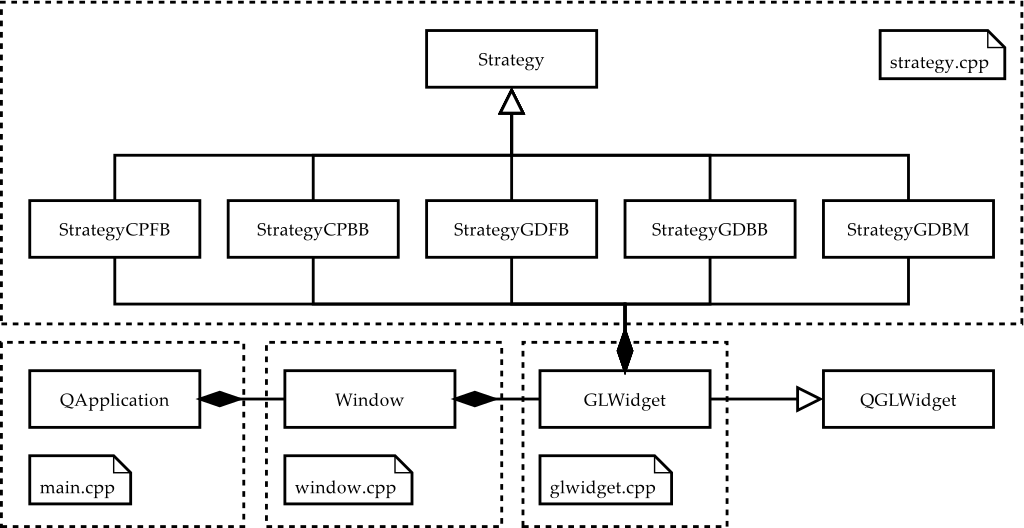
\includegraphics[width=0.9\textwidth]{fig/uml}
  \caption{UML diagram}
  \label{fig:uml}
\end{figure}

The basic structure of the application is shown in
figure~\ref{fig:uml}. A \lstinline|QApplication| is instantiated with
a \lstinline|Window| (\lstinline|main.cpp|). \lstinline|Window|
instantiates a \lstinline|GLWidget| (\lstinline|window.cpp|).
\lstinline|GLWidget| is a subclass of \lstinline|QGLWidget|, and it
sets up and runs OpenGL~ES code in its \lstinline|initializeGL()| and
\lstinline|paintGL()| functions (\lstinline|glwidget.cpp|). The
OpenGL~ES code is structured in a number of ``strategies'' inheriting
from a base class (\lstinline|strategy.cpp|), using the Template
Method pattern~\citep{erich95:-patterns}.

\section{Shaders}

\begin{figure}
  \centering
  \subfloat[Vertex shader]{
    \label{fig:vertexshader}
    \includegraphics[width=0.8\textwidth]{fig/vertexshader}
  }

  \subfloat[Fragment shader]{
    \label{fig:fragmentshader}
    \includegraphics[width=0.8\textwidth]{fig/fragmentshader}
  }

  \caption{OpenGL~ES shaders}
  \label{fig:shaders}
\end{figure}

Each strategy invokes a vertex shader and a fragment shader. Since
OpenGL~ES lacks a fixed-function pipeline, we must at the very least
specify a pass-through vertex shader and a texture sampling fragment
shader in order to render anything at all.

Both shaders take a number of data entries as input and return a
number of data entries as output. The vertex shader
(figure~\ref{fig:vertexshader}) takes a number of \emph{input
  attributes} and outputs a number of \emph{varyings}. The fragment
shader (figure~\ref{fig:fragmentshader}) takes the varyings as input
and outputs a \emph{color}.

Constant data used by shaders are globally available as
\emph{uniforms}. A special type of uniform is the \emph{sampler},
which represents a texture. It is used by the fragment shader for
looking up the color of a texture coordinate. As of OpenGL~ES 3.0,
texture lookup operations are also possible in the vertex
shader~\citep{aaftab14:-opengl-es}.

In the CPU-computed strategies, a pass-through vertex shader takes the
texture coordinate and position of each vertex and outputs them
unchanged as a varying and the OpenGL~ES attribute
\lstinline|gl_Position|. A texture sampling fragment shader takes the
texture coordinate as input and outputs the color of the texture at
that position.

In the GPU-accelerated strategies, transformation is performed in the
shaders. In the case of the vertex shader, the vertex position is
transformed before it is output to \lstinline|gl_Position|. In the
case of the fragment shader, the texture coordinate is transformed
before sampling the texture.

% This will be illustrated below.

\section{Compilation}

\begin{figure}[b]
  \centering
  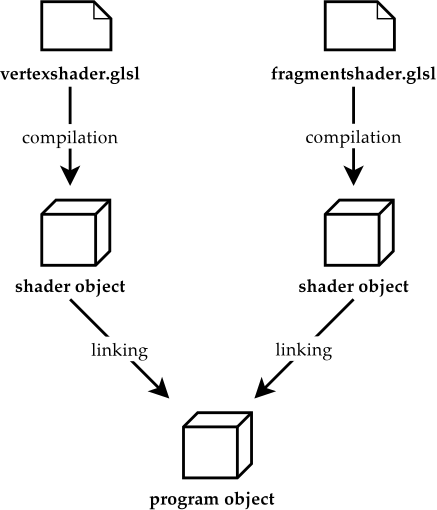
\includegraphics[width=0.5\textwidth]{fig/compilation}
  \caption{Shader compilation}
  \label{fig:compilation}
\end{figure}

When the implementation is initialized, the shaders are read from a
file on disk, parsed and compiled into a \emph{shader object} in
memory. The shader objects are then attached to and linked into a
\emph{program object} that performs the rendering
(figure~\ref{fig:compilation}). At this stage, vertex positions,
texture coordinates and textures can be allocated and bound to the
program object.

OpenGL~ES does not specify a binary format for program objects. This
is left to the vendor, which means that the format may change from one
driver version to another. If the \lstinline|glGetProgramBinary()| and
\lstinline|glProgramBinary()| functions are available, then a binary
representation can be saved to the file system to be reused later. In
this way, the cost of online compilation is avoided.

Our implementation does not cache the compilation step. Instead, time
measurements are postponed until \emph{after} OpenGL~ES has been
successfully initialized.

\section{Strategy 1: CPFB}

% \subsection{Grid}
% \label{sec:grid}

\begin{figure}[b]
  \centering
  \subfloat[Grid mesh]{
    \label{fig:gridmesh}
    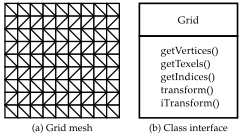
\includegraphics[height=0.3\textwidth]{fig/grid}
  }
  \quad\subfloat[Class interface]{
    \label{fig:gridclass}
    \includegraphics[height=0.3\textwidth]{fig/gridclass}
  }

  \caption{Grid class}
  \label{fig:grid}
\end{figure}

When computing the transformation on the CPU, we need to create a grid
mesh of $M \times N$ vertices -- a higher number means a more precise
transformation. This task is handled by the \lstinline|Grid| class
(\lstinline|grid.cpp|). The class encapsulates three arrays: an array
of vertex positions, an array of associated texture coordinates, and
an array of indices for drawing the triangles of the mesh. For
example, a grid of ten rows and ten columns is instantiated with
\lstinline|Grid(10, 10)|, while a simple square of four corners is
created with \lstinline|Grid(2, 2)|.

The mesh is constructed as a \lstinline|GL_TRIANGLE_STRIP|, with
alternating orientations of the inner triangles so that the whole
strip can be drawn in one pass (figure~\ref{fig:gridmesh}). Observe
that each point has a \emph{pair} of coordinates associated with it: a
vertex position in the range $[-1, 1]$ and a texture coordinate in the
range $[0, 1]$. The grid may be transformed by transforming the vertex
positions and holding the texture coordinates constant, or by
transforming the texture coordinates and holding the vertex positions
constant.

To perform a forward mapping transformation, we iterate through each
vertex position in the grid, transform it, and update the position. To
this end, the \lstinline|Grid| class provides an abstract interface
(figure~\ref{fig:gridclass}). The \lstinline|transform()| method takes
a \emph{functor class} as input. A functor class, in this context, is
merely a wrapper class for a function on vertex
positions.\footnote{Our functor classes are implemented as
  \emph{function objects}, that is, they overload the
  \lstinline|operator()| operator. C++11 also provides support for
  anonymous functions in the form of lambda expressions
  \citep{stroustrup13:-cpp-lang}, but these are difficult to compose
  in the way outlined in section~\ref{sec:implementationcpbb}.} By
implementing the transformation as such a class, we can pass it to the
\lstinline|Grid| class to perform transformation. (The vertex
positions themselves are represented by a \lstinline|Point| class with
an \lstinline|x| attribute and a \lstinline|y| attribute.)

After the grid has been transformed, it is ready for use and can be
textured by the input image. Its vertex positions and texture
coordinates are loaded as vertex attribute arrays, and become
available as input attributes for the vertex shader. Since we are not
using the GPU to accelerate the transformation, a simple a
pass-through vertex shader (listing~\ref{lst:vertexshader}) and a
texture sampling fragment shader (listing~\ref{lst:fragmentshader})
suffice.

In OpenGL~ES, if no default precision is specified, then the default
precision is \lstinline|highp| (the highest precision). It is possible
that the shaders may run faster or with a better power efficiency at a
lower precision. However, OpenGL~ES does not require the vendor to
support multiple precisions, so it is perfectly valid for an
implementation to ignore all qualifiers and perform the calculations
at the highest precision level.

\begin{lstlisting}[frame=lines,label=lst:vertexshader,caption=Pass-through vertex shader]
attribute vec2 a_texcoord;
attribute vec4 a_position;
varying vec2 v_texcoord;

void main() {
    gl_Position = a_position;
    v_texcoord = a_texcoord;
}
\end{lstlisting}

\begin{lstlisting}[frame=lines,label=lst:fragmentshader,caption=Texture sampling fragment shader]
varying vec2 v_texcoord;
uniform sampler2D s_texture;

void main() {
    gl_FragColor = texture2D(s_texture, v_texcoord);
}
\end{lstlisting}

\section{Strategy 2: CPBB}
\label{sec:implementationcpbb}

In the second CPU-computed strategy, we perform backward mapping
instead of forward mapping. That is, we hold the vertex positions
constant, and transform the texture coordinates instead.

To this end, the \lstinline|Grid| class provides the
\lstinline|iTransform()| method, which iterates through the grid's
texture coordinates. Recall that texture space's range of $[0, 1]$
differs from vertex space's range of $[-1, 1]$, so the method
implements algorithm~\ref{alg:coord} and converts between coordinate
spaces before and after transformation.

In this regard, our \lstinline|Functor| interface comes in handy.
Coordinate conversion, after all, is just another transformation, and
can be encapsulated in a functor class of its own. By defining a
\lstinline|chain()| method for composing functor classes, we can build
more complex transformations out of simpler transformations.
Transformation in texture space, for example, can be defined as the
composition of coordinate conversion and vertex transformation,
composed with reverse coordinate conversion (figure~\ref{fig:chain}).
Likewise, when we initialize the grid, we employ functor classes to
normalize vertex positions within the $[-1, 1]$ range and texture
coordinates within the $[0, 1]$ range.

\begin{figure}
  \centering
  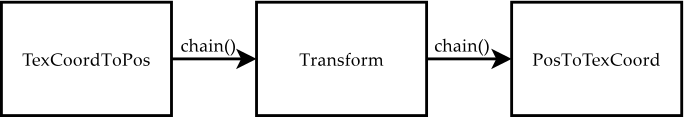
\includegraphics[width=0.8\textwidth]{fig/chain}
  \caption{Functor composition}
  \label{fig:chain}
\end{figure}

As before, once the grid has been transformed, it stays transformed.
The shaders are the same as for the previous strategy
(listings~\ref{lst:vertexshader}--\ref{lst:fragmentshader}).

\section{Strategy 3: GDFB}

The third strategy is a modification of the first strategy, but the
transformation is performed on the GPU instead. As before, we
instantiate an object of the \lstinline|Grid| class, but we
\emph{don't} invoke the \lstinline|transform()| method. Instead, we
leave it to the vertex shader to map each vertex to the transformed
position.

Listing~\ref{lst:vertexshadertransform} outlines the structure of the
vertex shader. The \lstinline|transform()| function implements our
choice of distortion model. Note that texture coordinates are passed
through unchanged.

\begin{lstlisting}[frame=lines,label=lst:vertexshadertransform,caption=Transformation in the vertex shader]
attribute vec2 a_texcoord;
attribute vec4 a_position;
varying vec2 v_texcoord;

// fish-eye transformation
vec4 transform(vec4 pos) {
    ...
}

void main() {
    gl_Position = transform(a_position);
    v_texcoord = a_texcoord;
}
\end{lstlisting}

\section{Strategy 4: GDBB}

In the backward mapping case, we transform the texture coordinates
instead. This step can be performed in the fragment shader prior to
sampling the texture. Since the fragment shader's texture coordinate
is the interpolated value between the vertices surrounding the
fragment's position, we don't need to create a detailed mesh
beforehand -- a ``grid'' consisting of four corners suffices.
Listing~\ref{lst:fragmentshadertransform} shows how the texture
coordinate is passed to \lstinline|transform()| before
\lstinline|texture2D()|.

\begin{lstlisting}[frame=lines,label=lst:fragmentshadertransform,caption=Transformation in the fragment shader]
varying vec2 v_texcoord;
uniform sampler2D s_texture;

// texture coordinates to vertex positions
vec2 texcoordtopos(vec2 tex) {
    ...
}

// vertex positions to texture coordinates
vec2 postotexcoord(vec2 pos) {
    ...
}

// fish-eye transformation
vec2 fisheye(vec2 pos) {
    ...
}

// transformation function
vec2 transform(vec2 tex) {
    return postotexcoord(fisheye(texcoordtopos(tex)));
}

void main() {
    gl_FragColor = texture2D(s_texture, transform(v_texcoord));
}
\end{lstlisting}

As in the CPU case, we must perform coordinate conversion before and
after transformation. This is done by the functions
\lstinline|texcoordtopos()| and \lstinline|postotexcoord()|. The
\lstinline|transform()| function encapsulates the invocation of these
functions and the \lstinline|fisheye()| function, which performs the
actual transformation.

Depending on the model parameters, it may be wise to check if the
transformed coordinate is within the $[0, 1]$ range, and return a
blank color if it isn't. This can done by substituting a custom
\lstinline|color()| function for the direct invocation of
\lstinline|texture2D()| (listing~\ref{lst:color}).

\begin{lstlisting}[frame=lines,label=lst:color,caption=Texture sampling function]
vec4 color(sampler2D texture, vec2 pos) {
    if(pos.x < 0.0 || pos.y < 0.0 ||
       pos.x > 1.0 || pos.y > 1.0) {
        return vec4(1.0, 1.0, 1.0, 1.0); // white
    } else {
        return texture2D(texture, pos);
    }
}

void main() {
    gl_FragColor = color(s_texture, transform(v_texcoord));
}
\end{lstlisting}

\section{Strategy 5: GDBM}
\label{sec:implementationgdbm}

The final strategy builds upon the previous to include custom
interpolation in the form of supersampling. This is done by sampling
the texture not once, but multiple times, and blending the values
together. The first task of the \lstinline|main()| method is to
compute the neighbor coordinates according to equations
(\ref{eq:ul}--\ref{eq:lm}):
\begin{lstlisting}[frame=lines,label=lst:neighbor,caption=Neighbor coordinates]
    vec2 v0 = vec2(v_texcoord.x - px/2.0,
                   v_texcoord.y + px/2.0);
    vec2 v1 = vec2(v_texcoord.x,
                   v_texcoord.y + px/2.0);
    ...
    vec2 v8 = vec2(v_texcoord.x + px/2.0,
                   v_texcoord.y - px/2.0);
\end{lstlisting}
Here, \lstinline|px| is the normalized size of a fragment (i.e., $1$
divided by the number of fragment rows or columns). The next step is
to transform these coordinates:
\begin{lstlisting}[frame=lines,label=lst:transformed,caption=Transformed coordinates]
    v0 = transform(v0);
    v1 = transform(v1);
    ...
    v8 = transform(v8);
\end{lstlisting}
We sample the texture at the transformed positions:
\begin{lstlisting}[frame=lines,label=lst:sample,caption=Transformed coordinates]
    vec4 c0 = color(s_texture, v0);
    vec4 c1 = color(s_texture, v1);
    ...
    vec4 c8 = color(s_texture, v4);
\end{lstlisting}
Then we can compute our interpolate value by blending these colors
together. For example, if \lstinline|blend9()| is a custom function
computing an unweighed average, then we can call
\lstinline|blend9(c0, c1, ..., c8)|.

We can also calculate a \emph{weighed} average, expressed in terms of
the kind of $3 \times 3$ kernel described in section~\ref{sec:gdbm}.
The \lstinline|mat3| data type is well suited to representing such a
kernel. First we write a general \lstinline|filter9()| function which
takes a set of colors, a kernel, a divisor, and returns a weighed
average:
\begin{lstlisting}[frame=lines,label=lst:filtering,caption=Filtering function]
vec4 filter9(vec4 c1, vec4 c2, ..., vec4 c9,
             mat3 kernel, float div) {
    return (c1 * kernel[0][0] +
            c2 * kernel[0][1] +
            ...
            c9 * kernel[2][2]) / div;
}
\end{lstlisting}
To this function we can for example pass a Gaussian kernel
(figure~\ref{fig:gaussian}):
\begin{lstlisting}[frame=lines,label=lst:gaussian,caption=Filtering function]
vec4 gaussian9(vec4 c1, vec4 c2, ..., vec4 c9) {
    mat3 kernel = mat3(1.0, 2.0, 1.0,
                       2.0, 4.0, 2.0,
                       1.0, 2.0, 1.0);
    return filter9(c1, c2, ..., c9, kernel, 16.0);
}
\end{lstlisting}
This will typically produce a crisper result than the unweighed
average.

The choice of kernel can be determined adaptively by specifying a way
to classify the image into concentric regions. For example,
classifying on the radius describes a circular area, while classifying
on the maximum transformed width or height describes a
``pincushion''-shaped area (illustrated in figure~\ref{fig:distance}):
\begin{lstlisting}[frame=lines,label=lst:distance,caption=Distance measure]
// radius
float distance() {
    return length(texcoordtopos(v_texcoord));
}

// maximum transformed width/height
float distance2() {
    vec2 vx = abs(fisheye(texcoordtopos(v_texcoord)));
    return max(vx.x, vx.y);
}
\end{lstlisting}
The appropriate kernel can be selected according to a given threshold:
\begin{lstlisting}[frame=lines,label=lst:adaptive,caption=Adaptive interpolation]
float r = distance();
if(r > 0.8) {
    gl_FragColor = sharpen9(c0, c1, ..., c8);
} else {
    gl_FragColor = gaussian9(c0, c1, ..., c8);
}
\end{lstlisting}
See section~\ref{sec:adaptive} for the visual results of adaptive
interpolation.

\section*{Summary}

Our implementation uses Qt for its surrounding framework, and is a
mixture of C++ and shader code. The CPU strategies leverages the
object orientation of C++ in order to structure the code. Both the
grid mesh and the transformation code are encapsulated in composable
classes.

The GPU strategies rely on shader code, which is not as structured.
Forward mapping is done in the vertex shader and backward mapping is
done in the fragment shader. In the latter case, no vertex grid is
necessary and a simple rectangle of four corner suffices.

When performing manual supersampling in the fragment shader,
OpenGL~ES' matrix data types can be used to represent filtering
kernels. By measuring the distance from the center, the image can be
divided into regions which are interpolated differently.

In the next chapter, we will measure the efficiency of these
strategies and compare their visual output.

% \section{Polar coordinates}

% Fish-eye transformations are expressed in polar coordinates $[r,
% \theta]$, not Cartesian coordinates $[x, y]$. We can convert between
% coordinate systems as shown in algorithm~\ref{alg:polar}. There are
% two conversion steps: from Cartesian coordinates to polar coordinates
% before transformation with a function $F(\mathbf{x})$, and then from
% polar coordinates to Cartesian coordinates after transformation.
% \begin{algorithm}[h]
%   \caption{Polar conversion}
%   \label{alg:polar}
%   \begin{algorithmic}
%     \STATE $[r, \theta] \leftarrow [\sqrt{x^2 + y^2}, \atantwo(y, x)]$ \COMMENT{convert to polar space}
%     \STATE $[r', \theta'] \leftarrow F([r, \theta])$ \COMMENT{transform coordinates}
%     \STATE $[x', y'] \leftarrow [r\cos{\theta}, r\sin{\theta}]$ \COMMENT{convert to Cartesian space}
%   \end{algorithmic}
% \end{algorithm}

% However, if the distortion is perfectly radial, only the $r$ parameter
% is affected by the transformation. We can simplify the computation by
% calculating the ratio $f = r'/r$ between the transformed radius and
% the untransformed radius, and using this value to scale the Cartesian
% coordinates. Algorithm~\ref{alg:scale} shows this more efficient
% approach.
% \begin{algorithm}[h]
%   \caption{Cartesian conversion}
%   \label{alg:scale}
%   \begin{algorithmic}
%     \STATE $r \leftarrow \sqrt{x^2 + y^2}$ \COMMENT{compute radius}
%     \STATE $f \leftarrow F(r)/r$ \COMMENT{compute ratio}
%     \STATE $[x', y'] \leftarrow [fx, fy]$ \COMMENT{transform coordinates}
%   \end{algorithmic}
% \end{algorithm}

% Of course, this is a specific property of radial transformations. In
% the general case of performing a polar transformation in texture
% space, \emph{two} conversions are necessary: to and from texture
% coordinates, and to and from polar coordinates, as shown in
% algorithm~\ref{alg:double}.

% \begin{algorithm}[h]
%   \caption{Double coordinate conversion}
%   \label{alg:double}
%   \begin{algorithmic}
%     \STATE $[x, y] \leftarrow [2(s - 1/2), 2(t - 1/2)]$ \COMMENT{convert to vertex space}
%     \STATE $[r, \theta] \leftarrow [\sqrt{x^2 + y^2}, \atantwo(y, x)]$ \COMMENT{convert to polar space}
%     \STATE $[r', \theta'] \leftarrow F([r, \theta])$ \COMMENT{transform coordinates}
%     \STATE $[x', y'] \leftarrow [r\cos{\theta}, r\sin{\theta}]$ \COMMENT{convert to Cartesian space}
%     \STATE $[s', t'] \leftarrow [x'/2 + 1/2, y'/2 + 1/2]$ \COMMENT{convert to texture space}
%   \end{algorithmic}
% \end{algorithm}

% \section{C++ versus OpenGL~ES}

% Forward mapping can be done in C++ (when constructing the mesh) or in
% OpenGL~ES (in the vertex shader). Backward mapping can also be done in
% C++ (when constructing the texture coordinates for the mesh) or in
% OpenGL~ES (in the fragment shader). We are thus left with four main
% ways of performing the transformation:
% \begin{enumerate}
% \item Forward mapping in C++
% \item Forward mapping in OpenGL~ES
% \item Backward mapping in C++
% \item Backward mapping in OpenGL~ES
% \end{enumerate}

% \section{Hybrid approaches}

% Hybrid approaches are also possible. For example, one drawback with
% performing the transformation in OpenGL~ES is that the transformed
% coordinates are computed over and over. A transformed mesh, on the
% other hand, can be computed once and used many times, for example in
% a succession of video frames. One way to combine the two approaches
% would be to compute the transformed mesh in OpenGL~ES rather than C++,
% by writing the results of a single OpenGL~ES pass to an array which is
% then re-used in future passes.

% \section{Anisotropic filtering}

% \section{Sharpening}

\chapter{Results}
\label{chap:results}

In this chapter, we compare the efficiency of the implementations. We
also compare built-in interpolation against manual interpolation.

\section{Setup}

The code was executed on a MacBook Air 13$''$ 2011 model with a 1,7
GHz Intel Core i5 processor, 4 GB 1333 MHz DDR3 RAM, and a Intel HD
Graphics 3000 graphics card with 384 MB memory, running OS X Yosemite
10.10.4.

Our test image is a photograph of $700 \times 700$~pixels
(figure~\ref{fig:testimage}).\footnote{Figure~\ref{fig:testimage} is
  an excerpt from the picture ``Many Lovers'' by Thomas Hawk, which is
  released under Creative Commons at
  \url{http://www.flickr.com/photos/thomashawk/102065939/}.} It has a
grid-like structure, which makes it easy to gauge the effects of the
transformation. It is also rich in detail, which makes it possible to
spot aliasing effects.

\begin{figure}
  \centering
  \includegraphics[width=0.7\textwidth]{fig/differentlovers}
  \caption{Test image}
  \label{fig:testimage}
\end{figure}

Our model of choice is the exponential model with $s = 0.76$ and
$\lambda = 3.8342$ (section~\ref{sec:exponential}). We will use
equation~(\ref{eq:expparam}) for forward mapping and
equation~(\ref{eq:logparam}) for backward mapping, which produces a
strong pincushion effect when applied to a regular image
(figure~\ref{fig:transformedimage}). In other words, our setup would
\emph{undistort} a photograph exhibiting a large degree of barrel
distortion.

\section{Measuring}

Execution time was measured with the Qt class
\lstinline|QElapsedTimer|, which attempts to use monotonic clocks if
possible. Its \lstinline|nsecsElapsed()| method returns the elapsed
time in nanosecond resolution if available. Although this precision is
available on the MacBook Air, our measurements are all in the
millisecond range. We execute each strategy $1000$~times. Then we
compute the average and the standard deviation of the measurements,
which are stored in a designated class \lstinline|Measurements|
(\lstinline|measurements.cpp|). For each execution, we reload the test
image into memory, forcing recomputation (listing~\ref{lst:reload}).
The image is loaded in \lstinline|GL_RGBA| format; some GPUs may
prefer a different format (e.g., \lstinline|GL_BGRA|), which forces
the driver to perform an automatic conversion.

% The reloading itself is not part of the measurement.

\begin{lstlisting}[float=b,frame=lines,label=lst:reload,caption=Reloading the image]
GLuint id = 0;
glDeleteTextures(1, &id);
glTexImage2D(GL_TEXTURE_2D, 0, GL_RGBA,
             img.height(), img.width(),
             0, GL_RGBA, GL_UNSIGNED_BYTE,
             img.constBits());
\end{lstlisting}

We measure the CPU strategies somewhat differently from the GPU
strategies. For the CPU strategies, the main work is done prior to the
rendering, when initializing the grid; the rendering itself is cheap.
For the GPU strategies, the opposite is the case: grid initialization
is negligible, and all the work is done during rendering. For the
former, we time grid transformation and rendering; for the latter, we
time first-pass rendering and subsequent rendering.

To achieve parity between the CPU strategies and the GPU strategies,
the grid is $700 \times 700$~vertices and the rendering surface is
$700 \times 700$~pixels. These dimensions make the number of vertices
equivalent to the number of fragments. Of course, since the GPU
strategies are processed in parallel, we should expect them to
outperform the linear CPU strategies. However, a less fine-grained
grid suffices in order to get good results, and we will experiment
with lowering the vertex count in section~\ref{sec:vertexcount}. For
the backward mapping strategies on the GPU, a simple rectangle of four
points is substituted for the grid.

\begin{figure}
  \centering
  \includegraphics[height=0.5\textwidth]{fig/differentlovers5}
  \caption{Transformed image}
  \label{fig:transformedimage}
\end{figure}

\section{Results}

\begin{table}
  \centering
  \begin{tabular}{@{}lllrr@{}}
    \toprule
    \multicolumn{3}{@{}l@{}}{Strategy} & \multicolumn{1}{l}{Average} & \multicolumn{1}{l}{Std.~deviation} \\
    \midrule
    1 & (CPFB) & grid transformation & 69.3 ms  & 7.8 ms  \\
      &        & rendering           & 28.3 ms  & 11.6 ms \\
    2 & (CPBB) & grid transformation & 89.8 ms  & 6.4 ms  \\
      &        & rendering           & 35.2 ms  & 5.6 ms  \\
    3 & (GDFB) & first rendering     & 25.5 ms  &         \\
      &        & next renderings     & 28.2 ms  & 3.6 ms  \\
    4 & (GDBB) & first rendering     & 33.4 ms  &         \\
      &        & next renderings     & 3.5 ms   & 0.9 ms  \\
    5 & (GDBM) & first rendering     & 293.8 ms &         \\
      &        & next renderings     & 5.8 ms   & 9.1 ms  \\
    \bottomrule
  \end{tabular}
  \caption{Time measurements}
  \label{tab:measurements}
\end{table}

\begin{figure}
  \centering
  \subfloat[Strategy 1 (CPFB): grid transformation]{
    \label{fig:time1}
    \includegraphics[width=0.45\textwidth]{fig/chart1}
  }
  \quad\subfloat[Strategy 2 (CPBB): grid transformation]{
    \label{fig:time2}
    \includegraphics[width=0.45\textwidth]{fig/chart2}
  }

  \subfloat[Strategy 3 (GDFB): rendering]{
    \label{fig:time3}
    \includegraphics[width=0.45\textwidth]{fig/chart3}
  }

  \subfloat[Strategy 4 (GDBB): rendering]{
    \label{fig:time4}
    \includegraphics[width=0.45\textwidth]{fig/chart4}
  }
  \quad\subfloat[Strategy 5 (GDBM): rendering]{
    \label{fig:time5}
    \includegraphics[width=0.45\textwidth]{fig/chart5}
  }

  \caption{Time series}
  \label{fig:timeseries}
\end{figure}

The results are listed in table~\ref{tab:measurements}. For the CPU
strategies, initializing and transforming the grid is considerably
more costly than rendering, but this operation needs only be done
once. Initialization is more costly for the backward mapping strategy
than for the forward mapping strategy. This goes to show that the
exponential equation~(\ref{eq:logparam}) is more costly to compute
than the logarithmic equation~(\ref{eq:expparam}). Thus, in this
context, the exponential model is \emph{not} a good choice for
backward mapping.

For the GPU strategies, forward mapping on the GPU is considerably
faster than on the CPU, as we expected. This suggests that the optimal
design for a forward mapping implementation would be to transform the
grid with a special ``initialization shader'' that is run only once
and whose results are saved for later use. The rendering time is the
same as for the CPU strategies.

For the backward mapping strategies on the GPU, an interesting pattern
emerges: the first rendering pass takes a long time, but subsequent
passes are very efficient. This pattern is illustrated in
figure~\ref{fig:timeseries}, which shows the five first measurements
from a test run of the strategies. For strategies 1--3, the
measurements are in the same range, but for strategies 4--5, there is
a sharp drop-off after the first pass. In other words, the
computations are cached, even when the texture is reloaded.

The first pass of strategy~5 (GDBM) is about an order of magnitude
more costly than the first pass of strategy~4 (GDBB). This is what we
would expect, since supersampling multiplies the workload with a
factor of nine. However, subsequent passes are an order of magnitude
cheaper for strategy~4, and \emph{two} orders of magnitude cheaper for
strategy~5. In other words, strategy~4 and strategy~5 perform in the
same range after the initial pass. Even more interestingly, this range
is an order of magnitude cheaper than the other strategies, including
strategy~3, which is also done on the GPU.

\section{Vertex count}
\label{sec:vertexcount}

\begin{figure}[b]
  \centering
  \includegraphics[width=0.9\textwidth]{fig/graph}
  \caption{Strategy 3 (GDFB) rendering time versus grid size}
  \label{fig:strategy3graph}
\end{figure}

The impact of vertex count on rendering time is illustrated in
figure~\ref{fig:strategy3graph}, which plots time measurements of
strategy~3 (GDFB). It is not until the grid resolutions falls below
$100 \times 100$ vertices that the efficiency becomes comparable to
that of the other two GPU strategies.

Moreover, the measurements of the CPU strategies in
table~\ref{tab:measurements} show that a high vertex count has a
significant impact on rendering time in and of itself, even when the
transformation is precalculated.

However, it is not necessary to employ a high-resolution grid in order
to see good results. Even a grid of as $50 \times 50$ vertices
produces adequate, if less precise results.

\section{Aliasing}

\begin{figure}
  \centering
  \subfloat[Bilinear interpolation]{
    \label{fig:detail1}
    \fbox{\includegraphics[clip,trim=300 300 300 300,width=0.4\textwidth]{fig/transformed}}
  }
  \quad\subfloat[Gaussian supersampling]{
    \label{fig:detail2}
    \fbox{\includegraphics[clip,trim=300 300 300 300,width=0.4\textwidth]{fig/transformedgaussian}}
  }

  \caption{Interpolation}
  \label{fig:interpolation}
\end{figure}

The impact of manual interpolation depends on the frequencies in the
test image. Figure~\ref{fig:interpolation} compares OpenGL~ES's built-in
bilinear interpolation against strategy~5 with a Gaussian kernel for a
detail of the test image. Manual interpolation produces a slightly
smoother result.

\begin{figure}[b]
  \centering
  \subfloat[Stripes image]{
    \label{fig:stripesimage}
    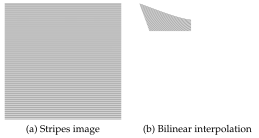
\includegraphics[width=0.3\textwidth]{fig/stripes}
  }
  \quad\subfloat[Bilinear interpolation]{
    \label{fig:stripestransformed}
    \includegraphics[width=0.3\textwidth]{fig/nofilter}
  }

  \caption{Stripes}
  \label{fig:Stripes}
\end{figure}

Aliasing effects can be brought to the fore by substituting a
high-frequency test pattern for the test image
(figure~\ref{fig:stripesimage}). In this case, pronounced aliasing
effects are unavoidable (figure~\ref{fig:stripestransformed}).

The effects are mitigated by supersampling
(figure~\ref{fig:supersamplingresults}). The softest output is
produced by supersampling with an averaging kernel of five values
(figure~\ref{fig:fiveaveragestripes}) or nine values
(figure~\ref{fig:nineaveragestripes}). Gaussian supersampling produces
a somewhat sharper result (figure~\ref{fig:gaussianstripes}). A
sharpening kernel retains the crispness of the lines, but pronounces
the aliasing effects, particularly in the center of the image
(figure~\ref{fig:sharpeningstripes}).

\begin{figure}
  \centering
  \subfloat[5-point supersampling]{
    \label{fig:fiveaveragestripes}
    \includegraphics[width=0.3\textwidth]{fig/blend5}
  }
  \quad\subfloat[9-point supersampling]{
    \label{fig:nineaveragestripes}
    \includegraphics[width=0.3\textwidth]{fig/blend9}
  }

  \subfloat[Gaussian supersampling]{
    \label{fig:gaussianstripes}
    \includegraphics[width=0.3\textwidth]{fig/gaussian9}
  }
  \quad\subfloat[Sharpening supersampling]{
    \label{fig:sharpeningstripes}
    \includegraphics[width=0.3\textwidth]{fig/sharpen9}
  }

  \caption{Supersampling results}
  \label{fig:supersamplingresults}
\end{figure}

\section{Adaptive interpolation}
\label{sec:adaptive}

To smooth out the aliasing effects in the center of the image while
mitigating the blurriness in the outer parts, we classify the image
into different regions. In figure~\ref{fig:distance1}, we classify
based on the calculated radius, which produces a number of concentric,
circular regions. In figure~\ref{fig:distance2}, we classify based on
the maximum transformed width or height, which produces a number of
concentric, transformed rectangles.

\begin{figure}
  \centering
  \subfloat[Radius]{
    \label{fig:distance1}
    \includegraphics[width=0.3\textwidth]{fig/distance1}
  }
  \quad\subfloat[Maximum transformed width or height]{
    \label{fig:distance2}
    \includegraphics[width=0.3\textwidth]{fig/distance2}
  }

  \caption{Distance measures}
  \label{fig:distance}
\end{figure}

Figure~\ref{fig:adaptive} shows the result with the maximum
transformed width or height as a distance measure, using gaussian
supersampling for the center of the image and sharpening supersampling
for the outer parts of the image. Regular bilinear interpolation is
used as a compromise between the two.

\begin{figure}[b]
  \centering
  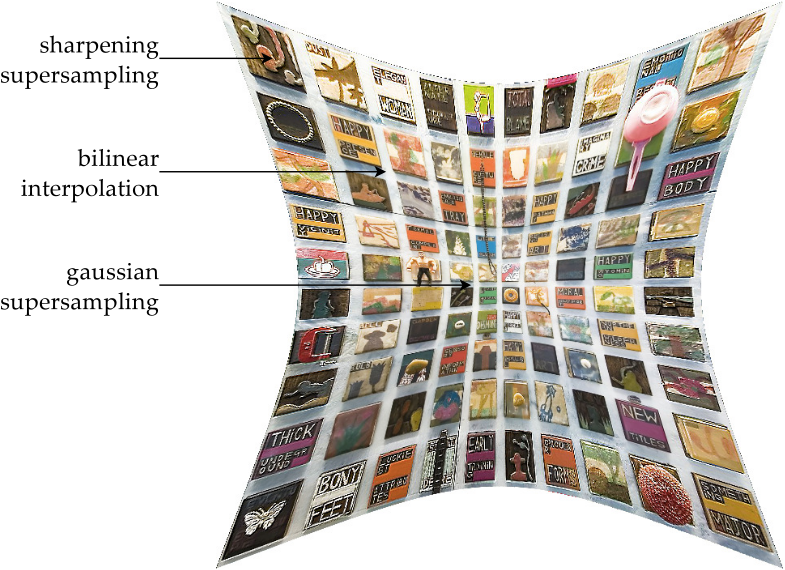
\includegraphics[height=0.5\textwidth]{fig/adaptive}
  \caption{Adaptive interpolation}
  \label{fig:adaptive}
\end{figure}

\section*{Summary}

The GPU strategies outperform the CPU strategies, and the backward
mapping GPU strategies outperform the others for repeated rendering
passes. Calculating the transformation in the fragment shader is
faster than calculating it in the vertex shader, even when the number
of vertices is lowered.

Supersampling adds an initial cost, but the efficiency is similar for
repeated passes. The visual impact depends on the image. In the case
of a photograph, supersampling a photograph produces a smoother
result. In the case of a test pattern, the aliasing effects are more
pronounced, and the smoothness depends on the choice of kernel.

Adaptive supersampling divides the image into regions that are
interpolated differently. This allows us to apply a smoothing filter
to oversampled areas and a sharpening filter to undersampled areas.
Such an interpolation strategies directly addresses the nonlinear
characteristics of a transformation such as barrel undistortion.

In the last chapter, we will sum up our findings and look into further
areas of investigation.

% Strategy  1  grid transformation:
% Average time:
%  69294312 ns (deviation:  7845479 )
%  (repetitions: avg =  69196144 , dev =  7846091 )

% 98161023 ns
% 75847145 ns
% 85910303 ns
% 82678322 ns
% 82723233 ns
% 84142230 ns
% 87850318 ns
% 82296324 ns
% 84722473 ns
% 82170556 ns
% ...

% Strategy  2  grid transformation:
% Average time:
%  89814016 ns (deviation:  6398383 )
%  (repetitions: avg =  89710304 , dev =  6399224 )

% 103725005 ns
% 157964832 ns
% 115325577 ns
% 109827233 ns
% 152447937 ns
% 93676366 ns
% 126584128 ns
% 94005177 ns
% 92384801 ns
% 86494482 ns
% ...

% Average time of strategy  1 :  "CPFB"
%  28282848 ns (deviation:  -2147483648 )
%  (repetitions: avg =  28230970 , dev =  11642287 )

% 51875856 ns
% 88045204 ns
% 88418109 ns
% 73432626 ns
% 49971227 ns
% 60321548 ns
% 67918603 ns
% 41845287 ns
% 60861875 ns
% 38670524 ns
% ...

% Average time of strategy  2 :  "CPBB"
%  35244812 ns (deviation:  5599937 )
%  (repetitions: avg =  35220112 , dev =  5599995 )

% 24701803 ns
% 36350018 ns
% 45899877 ns
% 30595841 ns
% 36825130 ns
% 36962432 ns
% 35365018 ns
% 41856985 ns
% 28913688 ns
% 35261398 ns
% ...

% Average time of strategy  3 :  "GDFB"
%  28218126 ns (deviation:  3607284 )
%  (repetitions: avg =  28192608 , dev =  3607373 )

% 25516110 ns
% 26409106 ns
% 25726665 ns
% 29330633 ns
% 24327955 ns
% 26646098 ns
% 26734121 ns
% 34201495 ns
% 20749674 ns
% 27797685 ns
% ...

% Average time of strategy  4 :  "GDBB"
%  3544175 ns (deviation:  993735 )
%  (repetitions: avg =  3510726 , dev =  994297 )

% 33448627 ns
% 4124590 ns
% 3656808 ns
% 3562690 ns
% 3329422 ns
% 3649040 ns
% 3543023 ns
% 3386574 ns
% 3378050 ns
% 3394308 ns
% ...

% Average time of strategy  5 :  "GDBM"
%  6137737 ns (deviation:  9106701 )
%  (repetitions: avg =  5843982 , dev =  9111445 )

% 293756411 ns
% 5920645 ns
% 5739885 ns
% 6064784 ns
% 6050247 ns
% 6225859 ns
% 6239838 ns
% 5845261 ns
% 6462072 ns
% 6535860 ns
% ...

\chapter{Conclusion}
\label{chap:conclusion}

% The interplay between transformation model and implementation strategy
% depends on whether the model is faster in the forward direction or the
% backward direction, and whether

In this thesis, we have studied and compared various approaches for
accelerating image transformation using OpenGL~ES. Our case has been
the undistortion of fish-eye distortion, a problem that can be modeled
in different ways. However, our results can be generalized to other
transformations as well.

In fitting a transformation model to an implementation strategy, we
can identify the following trade-offs:
\begin{enumerate}
\item \textbf{Precision:} Does the model produce accurate results? Is
  it a good fit to the error margins of the application, or does it
  introduce significant distortion of its own?
\item \textbf{Speed:} Is the model faster in the forward direction or
  in the backward direction? Is its efficiency offset by the chosen
  implementation strategy?
\item \textbf{Quality:} What interpolation method should be used? Does
  the input exhibit high frequencies that are prone to introduce
  aliasing effects? Should these effects be mitigated?
\end{enumerate}
Weighing these factors against each other, the best results by far are
produced by the backward-mapping strategies~4 (GDBB) and 5 (GDBM).
Even though the exponential model is slower in the backward direction
(and this is even more the case for other models, such as the
polynomial model), this is more than offset by the efficiency of the
strategies and the flexibility with regard to interpolation.

In other words: the model would have to be \emph{significantly} faster
in the forward direction than in the backward direction in order to
warrant a forward-mapping strategy over the backward-mapping
strategies mentioned above.

% Of course, nothing is perfect. Let us take a closer look at some of
% the weaknesses.

\section{Discussion}

In chapter~\ref{chap:introduction} we identified a number of
challenges: choosing a good model, selecting a fitting implementation
strategy, writing parallel code and achieving high-quality
interpolation. What is our assessment of these challenges?
\begin{itemize}
\item Among the several distortion models that are available, many
  deliver approximate results at low cost, but higher precision
  requires a more sophisticated model. Some models, like the
  polynomial model, can be orders of magnitude more expensive when
  applied in the reverse direction. The exponential model is a good
  compromise with comparable efficiency in both directions.
\item The cost of a precise model can be offset by an implementation
  strategy that is cheap, just like an imprecise model frees up
  resources for an expensive strategy. For the polynomial model, for
  example, a forward mapping strategy would be a better fit than a
  backward mapping strategy. For a model that is comparably efficient
  in both directions, such as the exponential model, a backward
  mapping strategy is superior in both efficiency and flexibility.
\item OpenGL~ES is eminently well suited to exploiting the
  parallelizable features of the problem. Data-parallel computing is
  achieved by implementing the transformation in terms of a vertex
  shader or fragment shader.
\item Although OpenGL~ES' built-in bilinear interpolation produces
  good results by itself, better results can be achieved by means of
  supersampling in the fragment shader. Such a method has the added
  benefit that it can be adapted to the transformation.
\end{itemize}
We conclude that OpenGL~ES is a good fit to the problem of
accelerating barrel undistortion, that the implementation adapts well
to the challenges raised, and that it is well supported by the
hardware of today.

\section{Further work}
\label{sec:furtherwork}

\begin{figure}
  \centering
  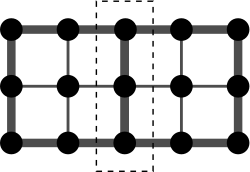
\includegraphics[width=0.4\textwidth]{fig/overlap}
  \caption{Overlapping samples}
  \label{fig:overlap}
\end{figure}

The multisampling shader makes nine texture accesses, most of which
are shared by the surrounding fragments, as shown in
figure~\ref{fig:overlap}. This means redundant accesses and coordinate
transformations, which are ``hopefully cached by the GPU'', in the
words of \citet{bjorke04:-filter}.

\citet{sigg05:-filtering} have presented a method for third-order
texture filtering which performs cubic filtering by building on linear
texture fetches, which considerably reduces the number of input
texture fetches. This could be used to optimize the
supersampling method presented in this thesis.

Furthermore, \citet{wexler05:-rasterization} have described a
supersampling technique for rendering images of arbitrary resolution
with arbitrarily wide user-defined filters and high sampling rates.
The image is divided into constant-size rectangular tiles in order to
support large supersampling rates and large final images.

To accelerate the code beyond what is possible with OpenGL~ES, we may
look into other frameworks. \citet{scarpino12:-opencl} goes into
detail on how to combine OpenGL with OpenCL in order to implement a
sharpening filter. In this setup, the filter is computed in parallel
by an OpenCL kernel, whose output is communicated to OpenGL by means
of a pixel buffer object. OpenGL is then used for rendering.

As OpenCL provides fine-grained memory handling where worker threads
may share data, this approach would make it possible to eliminate the
redundancy mentioned earlier. Indeed, it is similar to our CPU
strategies, except that the computations are not performed on the CPU,
but by a designated parallelization framework. However, such an
implementation would become considerably complex. As
\citeauthor{scarpino12:-opencl} puts it:
\begin{quote}
  OpenCL and OpenGL are both powerful toolsets, but no one has ever
  called them simple. Getting the two to work together is one of the
  most complex programming tasks I can think of~\dots\ I can't think
  of a harder topic related to
  OpenCL.\footnote{\citet{scarpino12:-opencl}, chapter 16: ``Textures
    and renderbuffers'', p.~349.}
\end{quote}
There is also the consideration that OpenCL is not as widely
supported, especially on mobile devices. A combined setup may pose
serious restrictions on portability and development environments.

\section*{Summary}

We have found OpenGL~ES to be well suited to the problem at hand. The
gains of parallelization are impressive, and a custom supersampling
strategy offers results above and beyond the standard interpolation
options. The supersampling strategy we have outlined is simple, but
adaptable.

The simplicity of OpenGL~ES comes with a disadvantage: it offers
little control over the parallelization. There is some redundancy in
the supersampling strategy that could be reduced by sharing memory
between worker threads. One way of exploring this possibility would be
to rewrite our OpenGL~ES shaders into OpenCL (or CUDA) kernels.

\appendix

\chapter{Source code}
\label{chap:code}

The source code is freely available from a Git repository. To obtain
the code, run the following command:
{\footnotesize
\begin{verbatim}
$ git clone https://epsil@bitbucket.org/mpg_papers/thesis-2015-vegard.git
\end{verbatim} }
To compile and run the code, run the included compilation script:
{\footnotesize
\begin{verbatim}
$ ./compile.sh
\end{verbatim} }
This will generate a Makefile (using \lstinline|qmake|), run the
Makefile, and then execute the resulting application.

% License

The code is freely available under the MIT
License.\footnote{\url{http://opensource.org/licenses/MIT}.}

\chapter{Matlab program}
\label{chap:matlab}

Matlab program for estimating model parameters:

\lstinputlisting{regression.m}

\backmatter{}

% \printbibliography

\bibliography{master} % (1 p.)

\bibliographystyle{plainnat}

\listoffigures
\listoftables
\lstlistoflistings
\listofalgorithms

\end{document}
